\documentclass[runningheads]{llncs}

\usepackage{natbib}

\usepackage[T1]{fontenc}

\usepackage{amsfonts}

\usepackage{amsmath}

\usepackage{graphicx}

\usepackage{svg}

\usepackage{acronym}

\usepackage{hyperref}

\usepackage{subfig}

\usepackage{multirow}


\newcommand{\topic}{Approaches for finding sample pairs in contrastive learning}
\newcommand{\authorA}{Klara M. Gutekunst}
\newcommand{\progcl}{ProGCL}
\newcommand{\curricularWeighting}{curricular weighting}

% If you use the hyperref package, please uncomment the following two lines
% to display URLs in blue roman font according to Springer's eBook style:
%\usepackage{color}
%\renewcommand\UrlFont{\color{blue}\rmfamily}
%\urlstyle{rm}
%
\begin{document}

%
\title{\topic}
%
\titlerunning{\topic}

\author{\authorA}
%
\authorrunning{\authorA}

\institute{University of Kassel, Germany\\
\email{klara.gutekunst@student.uni-kassel.de}}
%
\maketitle         
%
% include: speed bonus, no reloads, but no nesting, forces page break after and before input

% ---- Abstract ----
\begin{abstract}
    %The abstract should briefly summarize the contents of the paper in
    %150--250 words.

    Unsupervised learning techniques are of interest to many researchers, as they allow training models on data without any labels.
    \ac{ssl} is a subset of unsupervised learning, where labels are generated from unlabelled training data.
    \ac{cl} is a \ac{ssl} technique that is frequently used in representation learning.
    The representations of similar samples are supposed to be encoded within close range of each other, 
    while the representations of dissimilar samples are pushed apart.
    The selection of these dis-/similar pairs is subject to research.
    This paper reviews different approaches for finding sample pairs in \ac{cl}, with a focus on hard sample mining.
    
    \keywords{\acl{cl}  \and \acl{ssl} \and Hard sample mining.}
    \end{abstract}

% ---- Introduction ----
\section{Introduction}\label{sec:introduction}

\acf{ssl} is an unsupervised learning technique that allows training models on data without any labels.
The idea is to generate labels from the unlabelled training data contemplating a pre-text task.

Researchers usually select self-supervised pre-text tasks such that 
the targets can be generated without human annotations \citet{PIC_2020}.
The pre-text instance discrimination task considers each instance from the dataset its class.
A sample and its augmentations are considered positive pairs, 
while all other samples are considered negative pairs.
Hence, the model acquires an understanding of distinguishing between the instances and 
learns invariance to (image) transformations \citet{PIC_2020,swav_2020,local_aggr_2019,grape_2024,wang_understanding_2021}.

\textcolor{red}{\textbf{Research Question:} TODO \acf{cl}}

In order to explain why the proximity of generated samples to the anchor is relevant to the efficiency during training, 
one can consider a simple example in Euclidean space.
Imagine images as input to a \ac{nn}, which projects them onto $f_{\theta}(x) \in \mathbb{R}^d$, where $theta$ are the parameters of the \ac{nn}.

\begin{figure}[htbp]
    \centering
    \includesvg[width=300pt]{images/Hard_easy_samples_dist_effect_loss}
    \caption{svg image}
\end{figure}

% ---- main part ---- 
The selection of positive pairs ($x$, $x^+$) is subject to multiple papers, 
which propose different strategies.
In the case of unsupervised learning, generally, 
the positive sample $x^+$ is generated by applying a transformation to the anchor $x$.
Popular augmentation techniques include random cropping, color jittering, 
rotation and scaling \citet{ho_contrastive_2020,robinson_contrastive_2021}.

% PU learning
Another approach is to use so-called \ac{pu} learning, where learning is carried out 
on a set of positive and a set of unlabeled samples \citet{chuang_debiased_2020}.

% unsupervised learning
Simple selection techniques of negative samples include uniform sampling from the dataset or batch.
However, this approach is prone to two issues \citet{robinson_contrastive_2021,mining_potential_2024}:
\begin{enumerate}
    \item Selected samples are not necessarily hard negatives since the approach does not consider the embedding space proximity.
    \item Selected samples might actually belong to the same class as the anchor and thus, can be denoted \ac{fn}.
\end{enumerate}

% oracle learning
Some approaches use a so-called class oracle to boost the performance of the model.
If \acp{fn} \cite{grape_2024,curricular_weighting_2024,progcl_2022}, i.e. 
samples that belong to the latent class of the anchor but are considered negative, 
are sampled during hard negative mining, 
samples of the same class are pushed further apart in the embedding space. 
To avoid performance deterioration, this approach removes the \acp{fn} from the set of negative samples and thus, 
increases the performance of the model \citet{mochi_2020}.

\section{Related Work}\label{sec:related_work}

% sampling from distributions
Naturally, when using descriptive statistics to describe data, (empirical estimated) distributions play a crucial role.
Some researchers obtain their positive and negative samples from distributions.
Unfortunately, since \ac{cl} is a form of unsupervised learning, 
the true data distribution of the different classes is often not available.
Therefore, some scientists formulate assumptions or simplify the problem.
Possible assumptions include that the data distribution is uniform,
or approximating the positive sample distribution by sampling from a set of transformations 
or using the overall data distribution as a proxy for the negative sample distribution \citet{chuang_debiased_2020,robinson_contrastive_2021}.
In other cases, the class distributions are approximated using \acp{bmm} \citet{progcl_2022}.

Given the assumption that the data distribution is sufficiently well approximated, 
it is possible to consider probabilities of samples being \acp{fn} during the selection process of samples.
Needless to say, the goal is to avoid sampling \acp{fn} as negative samples.
To this end, scientists have proposed different strategies, which mostly boil down to 
incorporating the possibility of a potential negative sample being a \ac{fn} or \ac{tn} 
\citet{chuang_debiased_2020,robinson_contrastive_2021,progcl_2022}.


% augmentation strategies
Irrespective of its usage in the context of estimation of distributions, 
data augmentation is a common technique to create positive samples.
Often, an augmentation strategy is randomly sampled from a set of possible augmentations.
The motivation behind this is to increase the diversity of the positive samples 
in order to drive the model to learn features invariant to translations 
\citet{PIC_2020,swav_2020,local_aggr_2019,grape_2024,CL_temp_2021}.


% clustering/ distance
Since \ac{cl} objectives are often formulated in terms of distances or similarities between pairs of samples, 
the idea of using clustering techniques is a natural choice.
Intuitively, clusters of similar samples should be considered as positive samples and thus,
should be encoded close to each other.
Conversely, samples from different clusters should be encoded far apart.

Multiple methods have been proposed to generate samples via clustering.
Some ideas focus on high intra-cluster similarities to improve the alignment of the embeddings \citet{DRC_2020}.
Other ideas define different neighbour regions to condense representation within an inner radius 
while repelling samples from an outer radius \citet{local_aggr_2019}.
Another approach is to consider both Euclidean distance and semantic similarity to generate hard samples \citet{mining_manifolds_2018}.
Moreover, the \ac{pcl} technique defines positive samples as cluster centroids 
from one of the multiple clusterings for different numbers of clusters 
to encode the hierarchical structure of the data \citet{PCL_2021}.


% memory bank
Another prominent concept is the usage of memory banks to store embeddings of the data.
\citet{mochi_2020} fill these memory banks with embeddings of negative samples 
and propose two approaches for generating new hard negatives: 
Two of the most difficult samples currently stored in the memory bank are randomly selected and mixed.
The second approach is to use only one of the existing negative samples and 
mix it with the anchor to create a new sample.

\citet{progcl_2022} propose a method that extends the idea of \citet{mochi_2020} by weighting randomly selected negative samples 
with their relative similarity to the anchor when mixing them to create more difficult negative samples.

It is also possible to use the memory bank to store the embeddings of the positive samples.
Similarly, either randomly chosen samples can be used individually or 
the samples can be weighted by their hardness during loss calculation \citet{mining_potential_2024}.


% other work
% EM-algorithm
Multiple approaches, including \ac{drc}, \ac{pcl} and \progcl{}, use the \ac{em} algorithm 
to reduce computational costs or to find solutions via approximations.
Both \ac{drc} \citet{DRC_2020} and \progcl{} \citet{PCL_2021} are clustering-based methods 
while \progcl{} \citet{progcl_2022} is a distribution-based method.

% temperature
Since most approaches use a temperature parameter to control the hardness of the negative samples, 
\citet{CL_temp_2021} and \citet{grape_2024} investigate the impact of the temperature on the performance of the model.
They find that the \ac{cl} loss function optimizes hard samples by penalizing them according to their hardness.
If the temperature is small, only the closest points are penalized and others are not.
This can result in a uniformly distributed embedding space.

% curriculum learning
\citet{curricular_weighting_2024} propose a curriculum learning approach to generate hard negative samples.
They outline why curriculum learning is beneficial for \ac{cl} and how it can be implemented.

% data scheduling
% \citet{PIC_2020} propose a method to schedule the data for training 
% to reduce the periods within which a sample is not considered for training.


\section{Sampling techniques}\label{sec:sampling_techniques}

The following sections present different sampling techniques for 
positive and negative samples in \ac{cl} as displayed in \autoref{tab:overview}.
Firstly, sampling strategies based on distributions are discussed.
Secondly, clustering-based sampling techniques are presented and 
the impact of temperature on the sampling process is discussed.
Then, a technique relying on a memory bank is introduced.
Finally, curricular weighting is discussed. 
The latter is a technique that is not directly of interest in terms of sample generation 
but in terms of sample selection during training.

% Please add the following required packages to your document preamble:
% \usepackage{multirow}
\begin{table}[]
    \caption{Overview of \acs{cl} techniques}
    \label{tab:overview}
    \begin{tabular}{|l|l|l|}
    \hline
    \textbf{Category}                                   & \textbf{Name}                             & \textbf{Authors} \\ \hline
    \multirow{3}{*}{Distribution} & \acs{pu} approximation                          & \citet{chuang_debiased_2020}                \\ \cline{2-3} 
    \multicolumn{1}{|c|}{}                              & Choosing the hardness of negative samples     & \citet{robinson_contrastive_2021}                \\ \cline{2-3} 
    \multicolumn{1}{|c|}{}                              & ProGCL (Graphs)                               & \citet{progcl_2022}                \\ \hline
    \multirow{5}{*}{Clustering}                         & \acs{drc}                                       & \citet{DRC_2020}                \\ \cline{2-3} 
                                                        & \acs{swav}                                      & \citet{swav_2020}                \\ \cline{2-3} 
                                                        & \acs{la}                                       & \citet{local_aggr_2019}                \\ \cline{2-3} 
                                                        & Mining on manifolds                           & \citet{mining_manifolds_2018}                \\ \cline{2-3} 
                                                        & \ac{pcl}                                      & \citet{PCL_2021}               \\ \hline
    \multirow{2}{*}{Memory bank}                             & \acs{mochi}                                     & \citet{mochi_2020}                \\ \cline{2-3} 
                                                        & Extension of \acs{mochi}                        & \citet{progcl_2022}                \\ \hline
    Sample selection                                              & Curricular weighting                          & \citet{curricular_weighting_2024}               \\ \hline
    \end{tabular}
    \end{table}

% distributions

\subsection{Sample from distributions}
\label{subsec:SampleViaDistribution}

% Intuition
Assuming the distribution $p$ of a variable $x$ is known, i.e. $x \sim p$, it is possible to sample from it.
Sampling can either be done directly or 
via approximation schemes such as rejection sampling and Monte Carlo sampling \citep{robinson_contrastive_2021}.
However, in the context of \ac{cl}, the true data distribution of the different classes is often not available 
due to the nature of unsupervised learning scenarios.
Therefore, some scientists formulate assumptions or simplify the problem.

% mathematical foundation
%Positive pairs ($x$, $x^+$) are considered to originate from the same class.
% Let $\rho(c), c \in \mathcal{C}$ be the distribution over the latent classes and 
% let $h: \mathcal{X} \rightarrow \mathcal{C}$ be the ground truth assigning class labels $c \in \mathcal{C}$ to inputs $x \in \mathcal{X}$.
% Hence, $x \sim x'$ if $h(x) = h(x')$ \citet{robinson_contrastive_2021,chuang_debiased_2020}.

% PU learning
\subsubsection{\ac{pu} approximation}\label{subsec:pu_approximation}

\citet{chuang_debiased_2020} assume a \ac{pu} learning scenario, 
where positive samples and an unlabeled image dataset $p(x)$ are available.
Since positive samples may not be available in reality, 
the positive distribution $p^+$ is mimicked by data augmentations.

\citeauthor{chuang_debiased_2020}'s goal is to sample \acp{tn}.
They denote sampling bias the phenomenon of sampling \acp{fn} as illustrated in \autoref{fig:sampling_bias}a.
When randomly sampling negative samples from the data distribution $p(x)$ 
a negative sample can inherently belong to the same latent class as the anchor.
The negative effect of sampling bias on the model's performance is illustrated in \autoref{fig:sampling_bias}b.
Consequently, they propose a debiased contrastive objective that corrects for sampling \acp{fn} 
%i.e., the selection of negative samples that have the same label as the anchor, 
in an unsupervised scenario.
The idea is to generate positive samples using augmentations,
to sample negative samples $x^-$ from the data distribution $p(x)$
and to add a correction term for \acp{fn} in the loss function.

\begin{figure}%
    \centering
    \subfloat[\centering Visualization of sampling bias similar to \citet{chuang_debiased_2020}. Sampling $x_i^-$ from $p$ can result in \ac{fn}.]
    {{\includegraphics[width=5cm]{images/sampling_bias.png} }}%
    \qquad
    \subfloat[\centering Negative influence of sampling bias on accuracy from \citet{chuang_debiased_2020}.]{{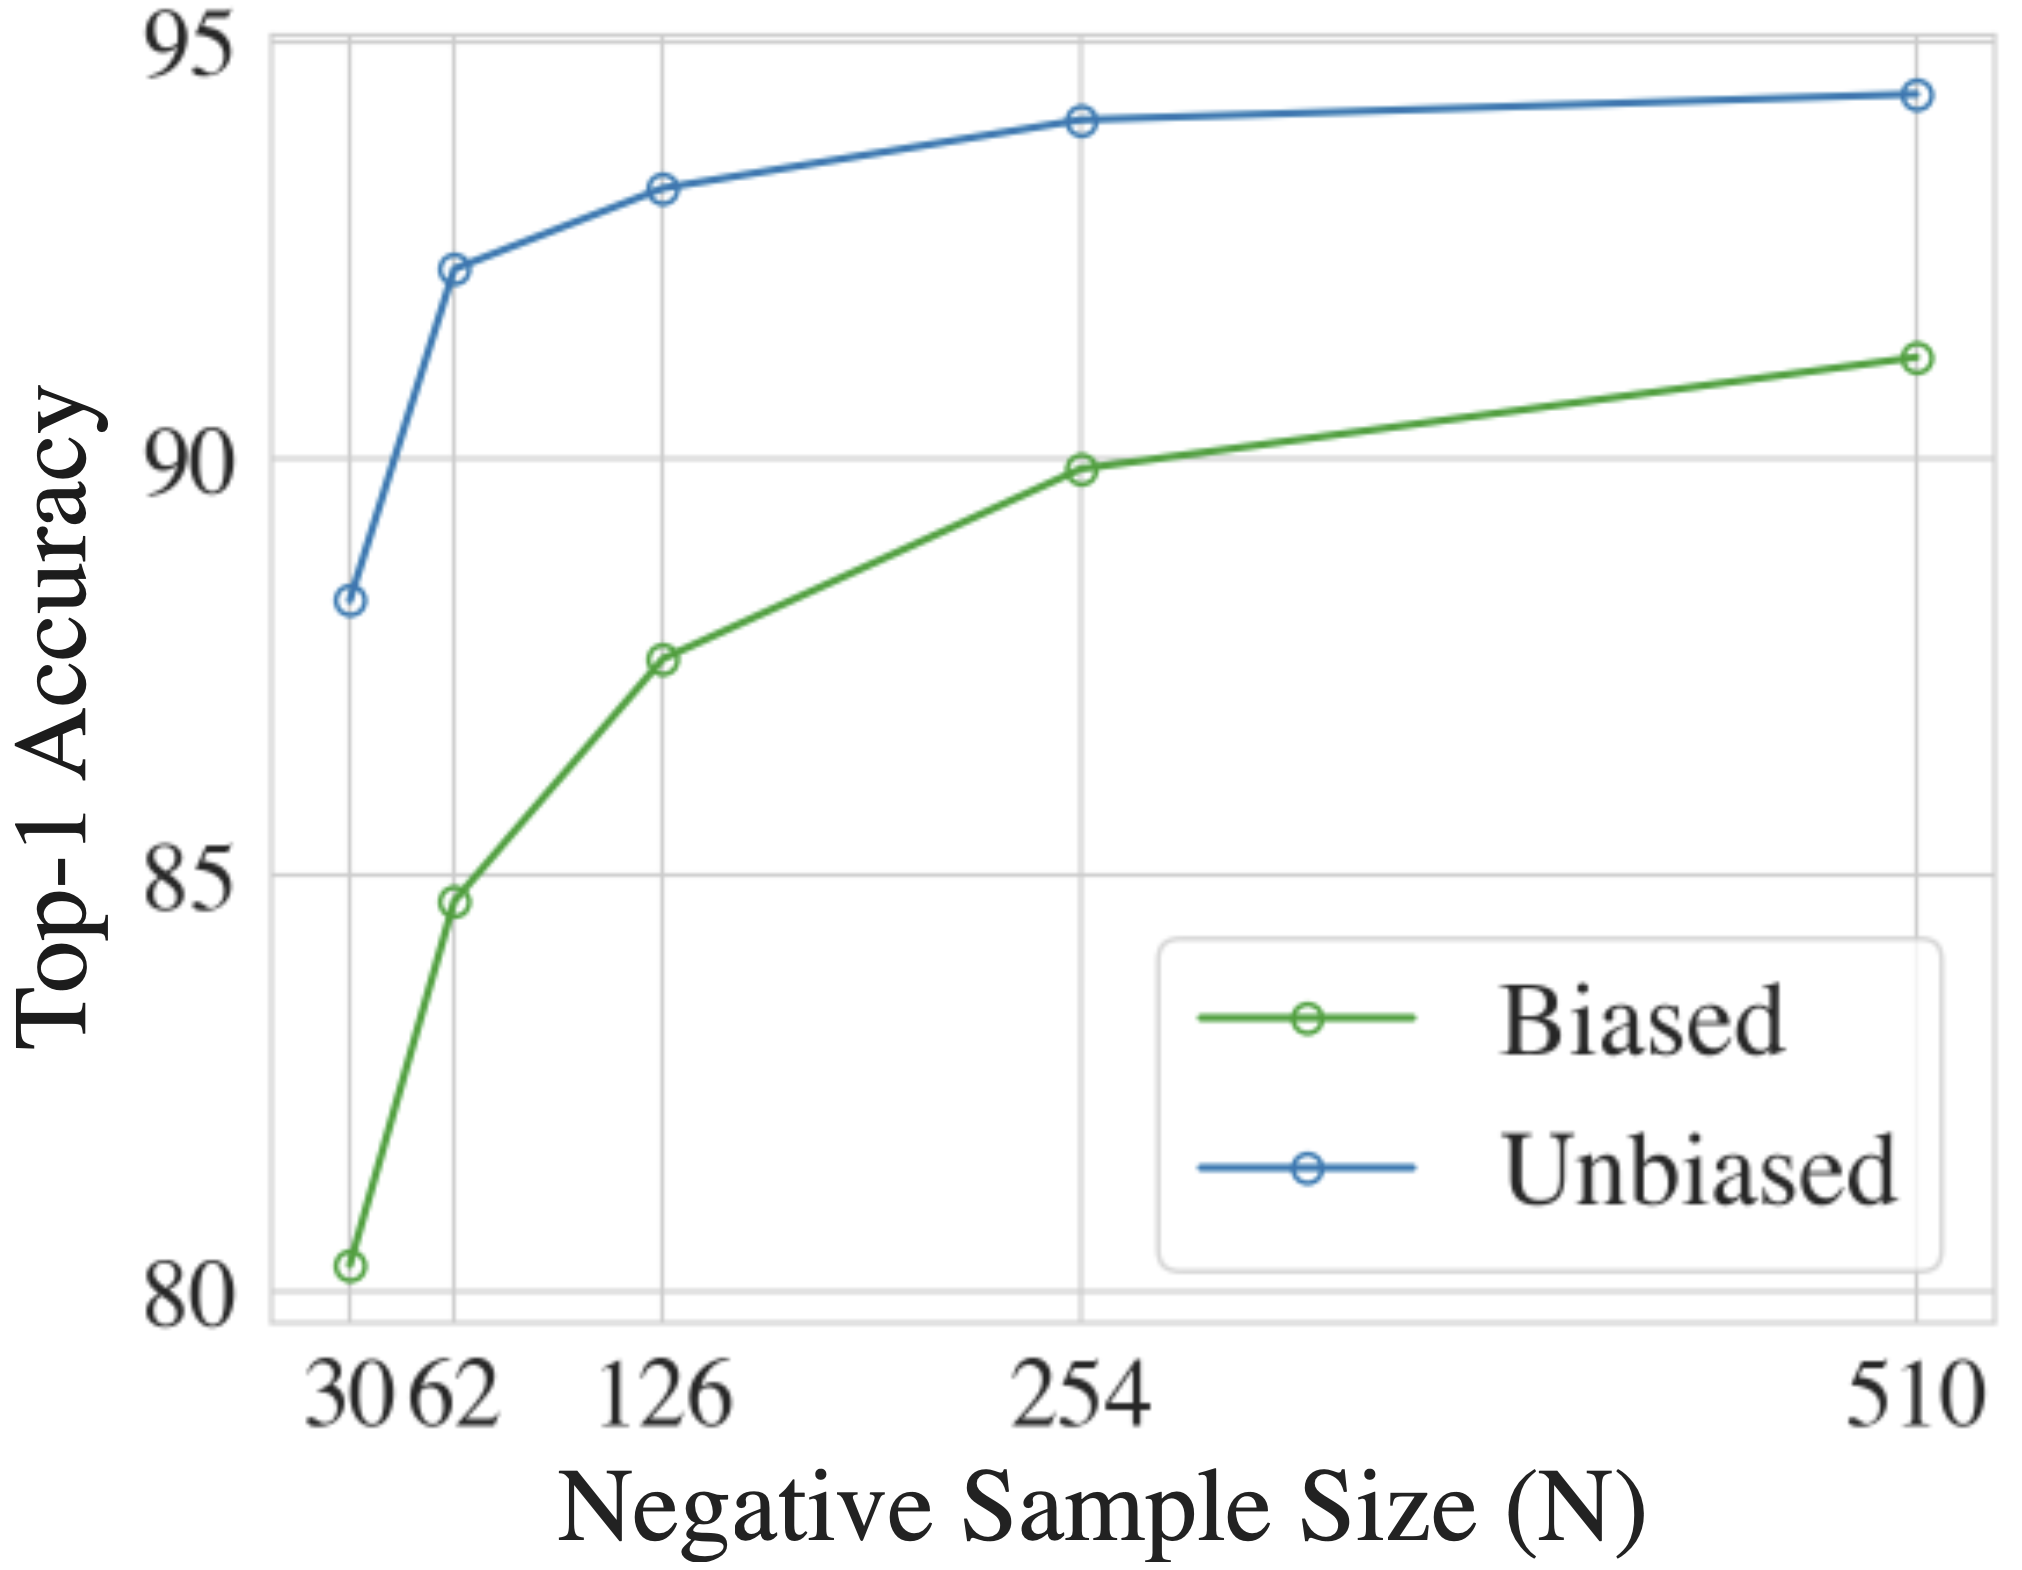
\includegraphics[width=5cm]{images/debiased_sampling_accuracy.png} }}%
    \caption{Visualization of sampling bias and its effect on the model's performance.}%
    \label{fig:sampling_bias}%
\end{figure}


% Choose hardness (Robinson)
\subsubsection{Choosing the hardness of negative samples}\label{subsec:choose_hardness}

\citet{robinson_contrastive_2021} 
extend \citet{chuang_debiased_2020}'s approach to sampling from distributions of image data.
Again, sampling from the positive sample distribution is approximated by sampling from a set of transformations
while negative samples $x^-$ are obtained by sampling from the data distribution $p(x)$.

\citet{robinson_contrastive_2021} introduce the concentration parameter $\beta$ 
to enable user-specific hardness of the negative samples.
$\beta$ is a multiplicative factor for the similarity, i.e. dot product $\beta f(x)^\text{T}f(x^-)$, of two sample feature space representations.
Hence, large values of $\beta$ lead to sampling very hard negative samples and thus, 
increase the risk of sampling \acp{fn}.


% graphs (ProGCL)
\subsubsection{Graphs}\label{subsec:graph_distribution}

Another prominent data structure is graphs, which can model 
social networks, citation networks, or knowledge graphs.
\citet{progcl_2022} propose an approach to mine negative samples for \ac{cl} on graphs called \progcl{}. 
As a motivation, the authors compare the similarity between the anchor and \acp{tn} 
to the similarity between the anchor and \acp{fn} 
across multiple datasets for both conventional \ac{cl} and \ac{gcl}.
The resulting distributions shown in \autoref{fig:sim_t_f_neg_image_graph} 
indicate that for \ac{gcl} the majority of highly similar negative samples are \acp{fn}, 
while for conventional \ac{cl} there seems to be no clear trend.
Moreover, the authors found that both the \ac{tn} and \ac{fn} distributions are best modeled by a beta mixture model %\acl{bmm} 
since it is able to fit the skewed empirical distribution.
The distribution is fitted using the \ac{em} algorithm on a subset of samples for a reduction of computational costs.

\begin{figure}%
    \centering
    \subfloat[\centering CIFAR-10 (Image)]
    {{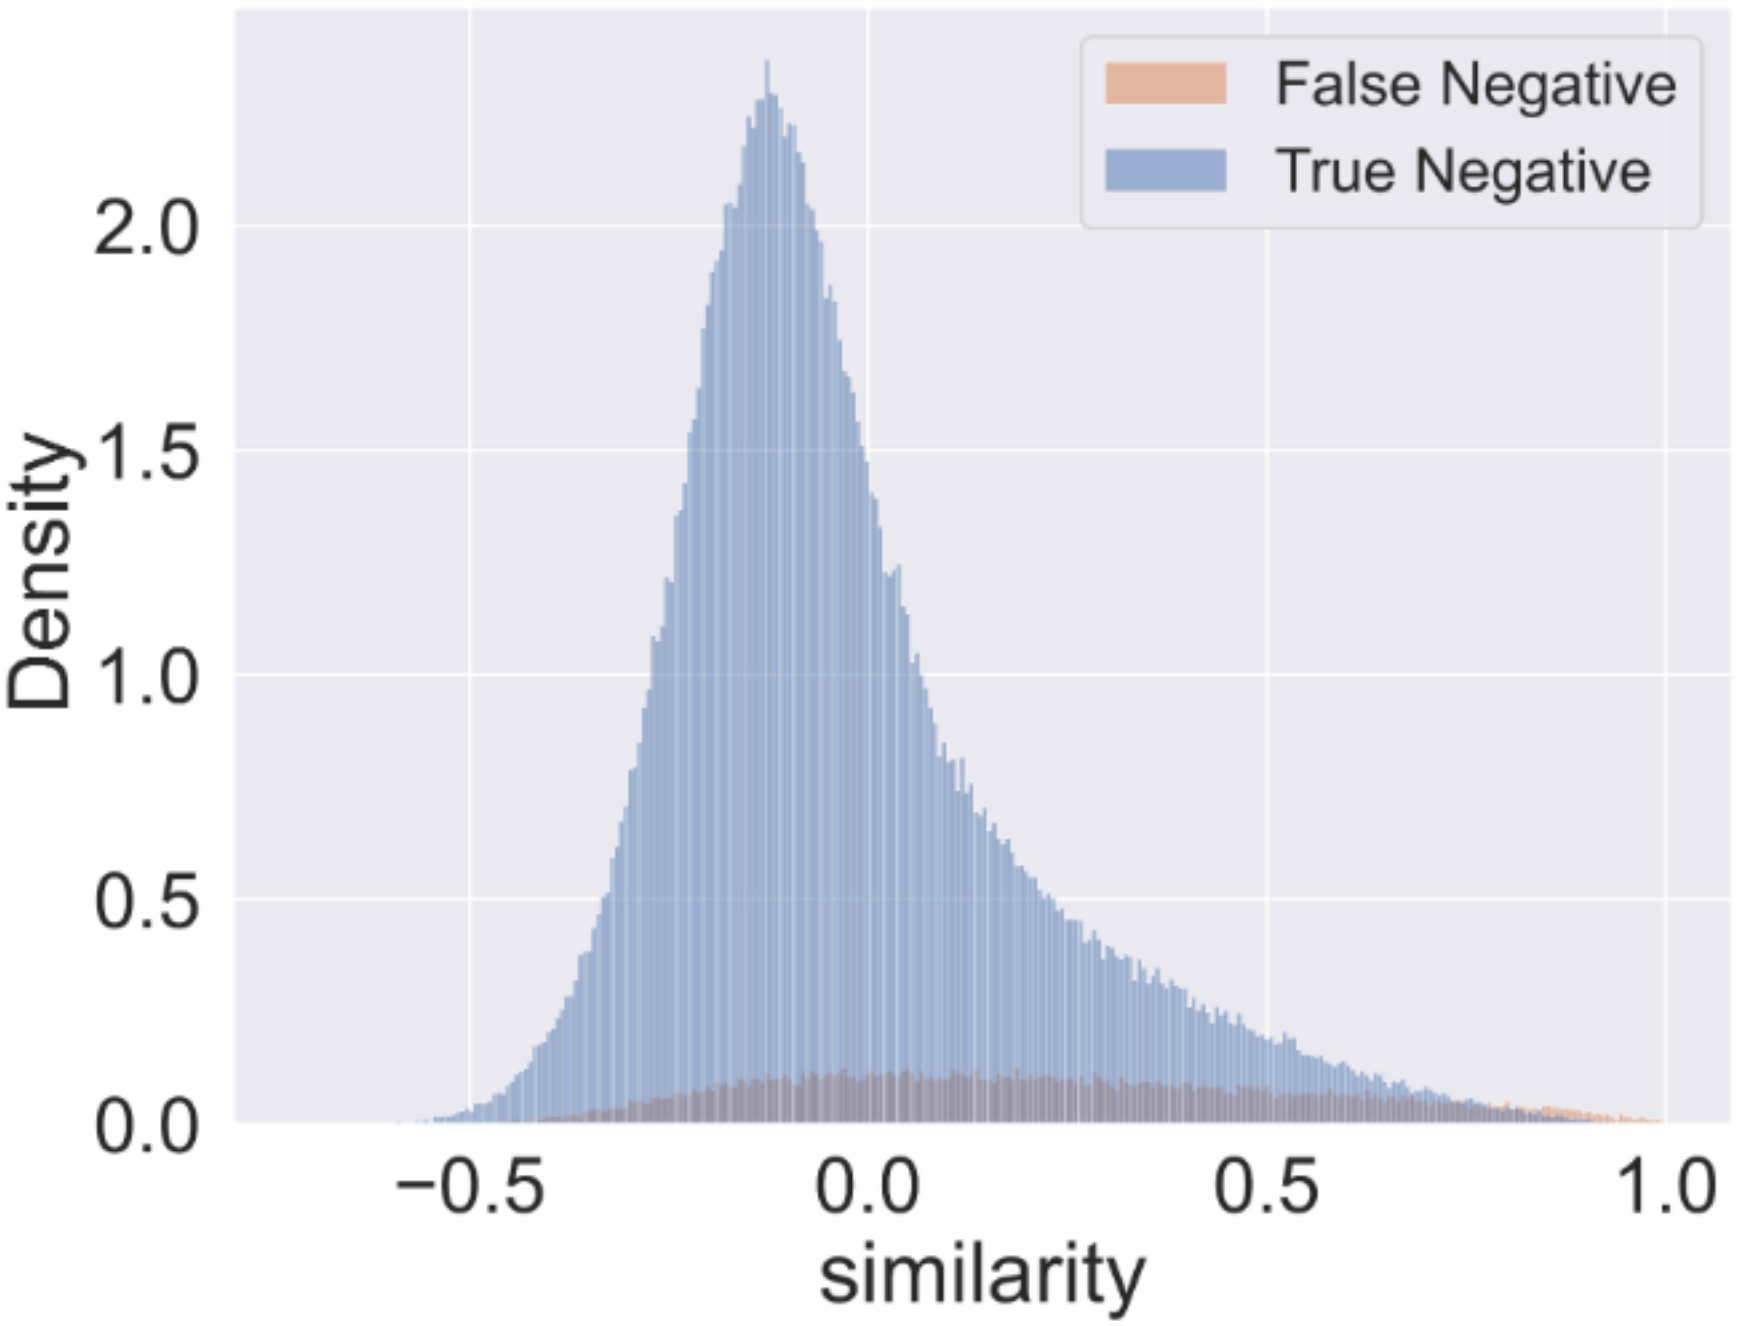
\includegraphics[width=4.8cm]{images/sim_negatives_image_data.png} }}%
    \qquad
    \subfloat[\centering Coauthor-CS (Graph). Most similar negative samples are \acp{fn}.]
    {{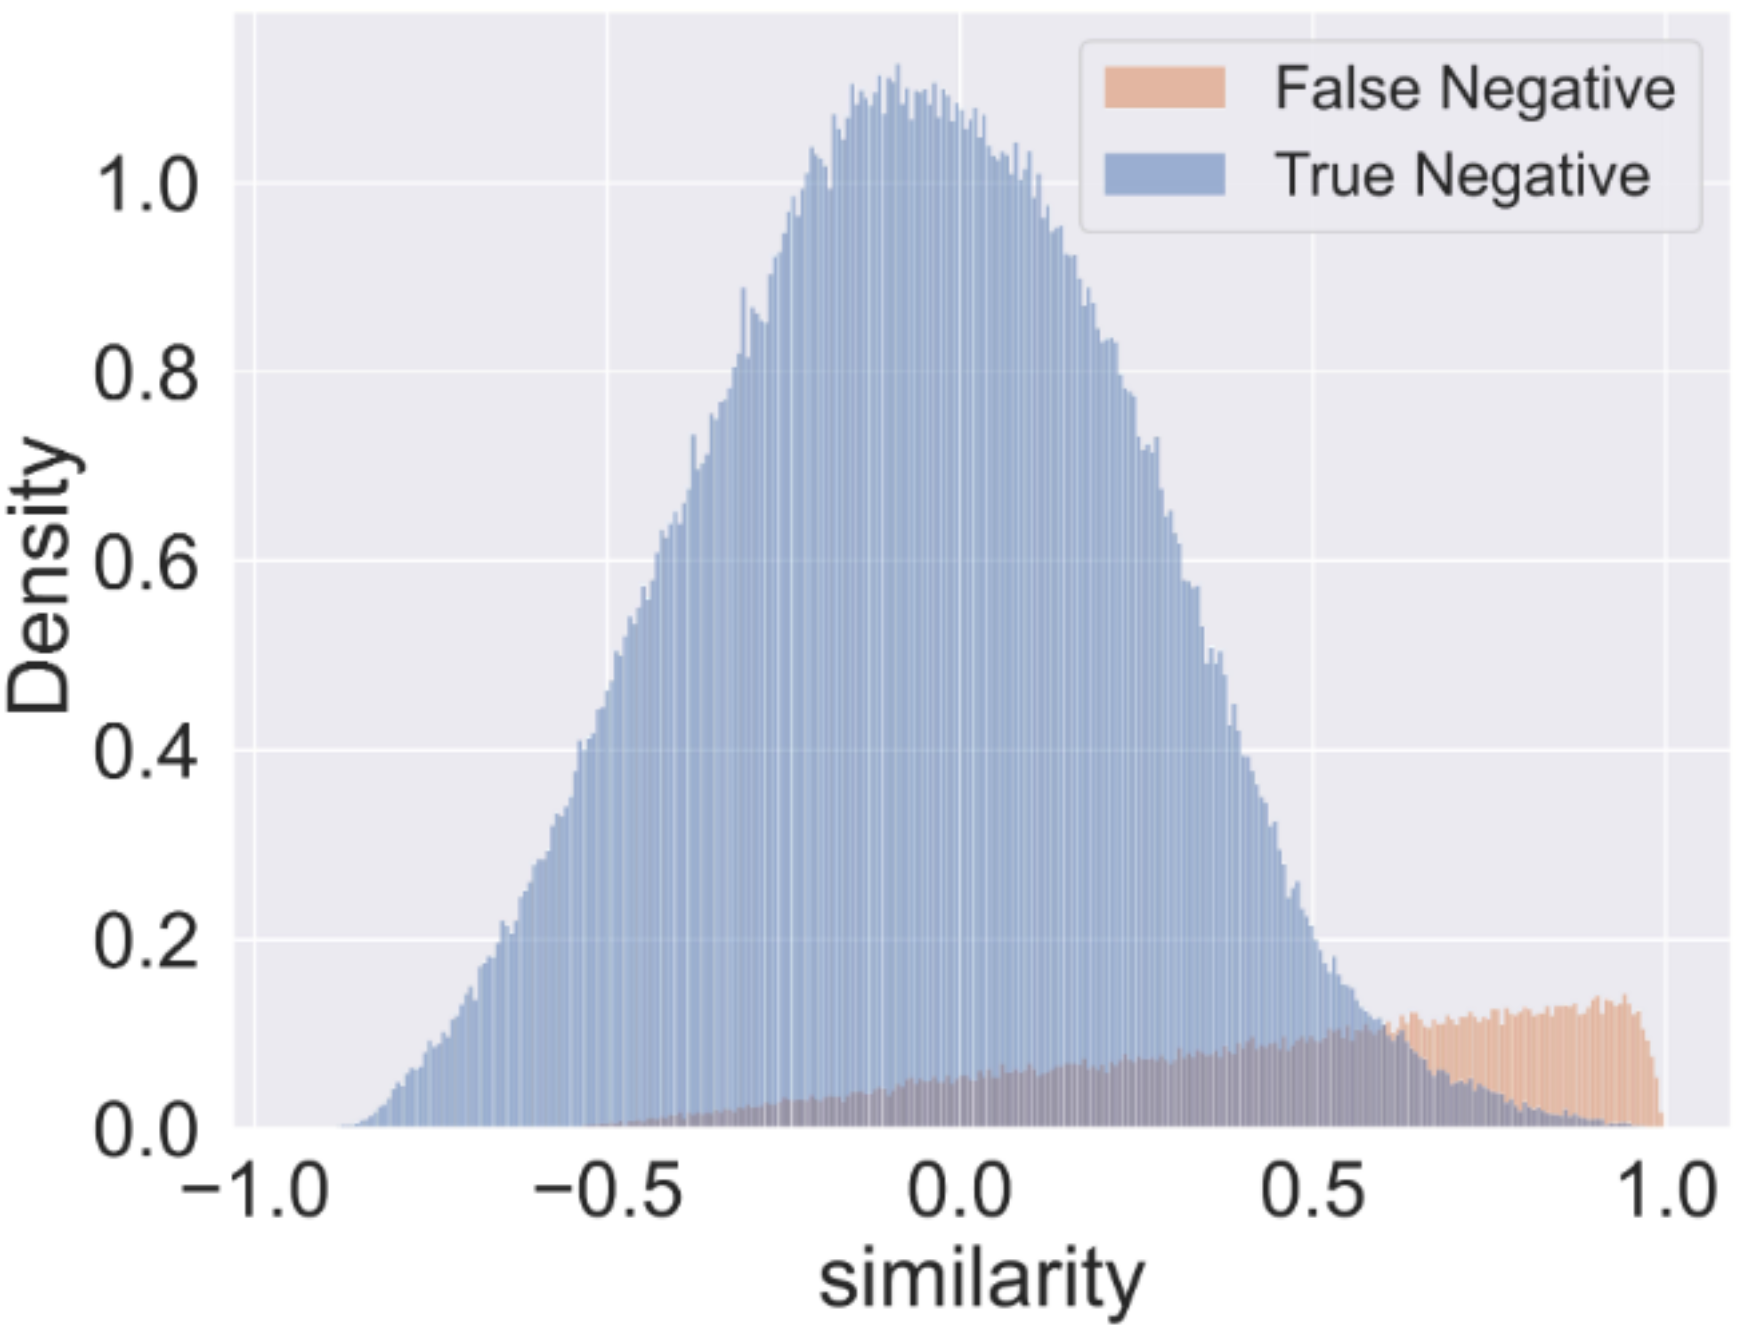
\includegraphics[width=5.2cm]{images/sim_negatives_graph_data.png} }}%
    \caption{Histogram of similarity between anchor and negative samples for \ac{cl} and \ac{gcl} from \citet{progcl_2022}.
    Blue denotes the empirical distribution of the \acp{tn}, while orange denotes \acp{fn}.}%
    \label{fig:sim_t_f_neg_image_graph}%
\end{figure}

% scheme 1: ProGCL-weight
Building on this observation, the authors propose incorporating both the probability of a sample being a \ac{tn} and 
the sample's similarity to the anchor, referred to as its hardness, into the negative sample selection process. 
It is important to note that the anchor is not a cluster center, 
but rather the sample from which augmentations are derived.

% scheme 2: ProGCL-mix (cf. MoCHi)


% clustering/ distance
\subsection{Sample via clustering}
\label{subsec:SampleViaClustering}
% easy approaches
% DRC (AF, AP & reg losses)
\subsubsection{\ac{drc}}\label{subsubsec:drc}

\citet{DRC_2020} propose a method called \ac{drc} 
that aims to address the issue of high intra-class diversities in existing deep clustering methods.
Even though the \ac{ap} can be similar for different samples, their \ac{af} can be different 
as illustrated in \autoref{fig:drc_af_ap}.
They claim that existing methods cluster dissimilar feature space representations \ac{af} together,
due to the usage of the maximum sensitivity of the softmax function used during cluster assignment.
\ac{drc} aims to address this issue by considering both the \ac{af} and the \ac{ap} during clustering.

\begin{figure}[h] % h = here, t = top, b = bottom, p = page of floats
    \centering
    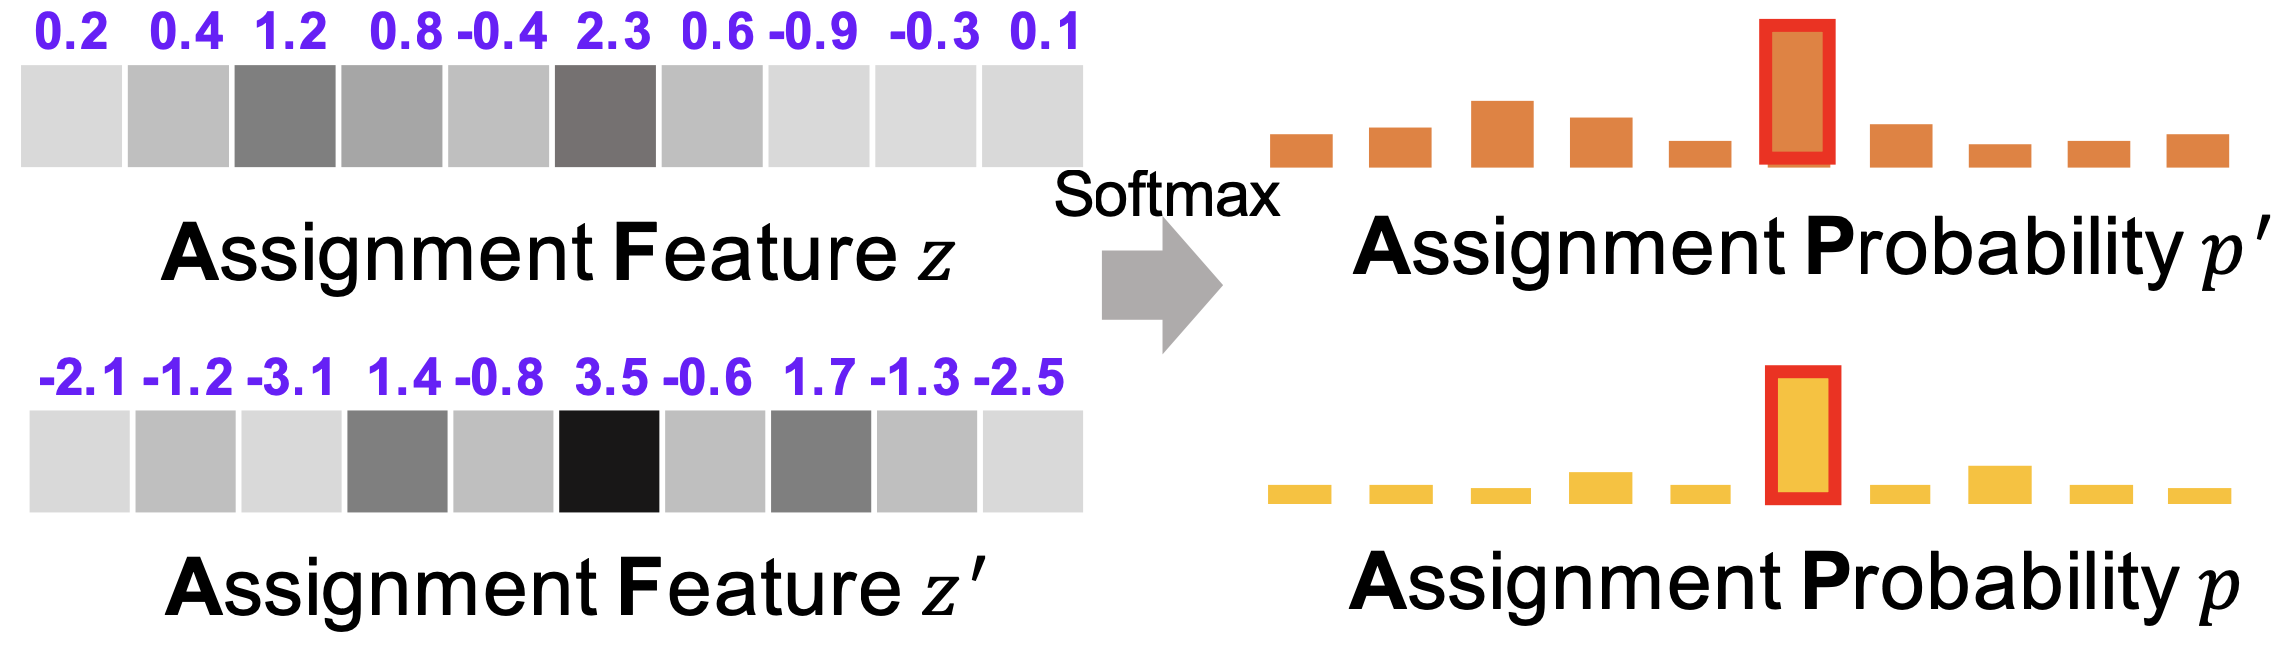
\includegraphics[width=300pt]{images/DRC_af_ap.png}
    \caption{Similar \ac{ap} values for different samples, but different \ac{af} values from \citet{DRC_2020}.
    Cluster assignment based on only \ac{ap} values can result in high intra-cluster diversities.}
    \label{fig:drc_af_ap}
\end{figure}

The \ac{af} $z_i$ are obtained from a \ac{cnn} with a fully connected layer, i.e. $z_i = f_\theta(x_i)$.
The \ac{ap} are obtained from the softmax function from \eqref{eq:ap}. 
Each sample $x_i$ is assigned to the cluster $j$ with the highest \ac{ap} value $p_{ij}$.
Optimally, the samples of a certain latent class should belong to the same cluster.

\begin{equation}
    p_{ij} = \frac{e^{z_{ij}}}{\sum_{K}^{t=1}e^{z_{it}}}, j \in \left[1,K\right]
    \label{eq:ap}
\end{equation}

\citeauthor{DRC_2020} present the loss function $\mathcal{L} = \mathcal{L}_{AF} + \mathcal{L}_{AP}  + \lambda \mathcal{L}_{CR}$  consisting of three terms.
The first term $\mathcal{L}_{AF}$ is the \ac{af} loss, which enforces similar representations of the sample and its positive transformation.
The second term $\mathcal{L}_{AP}$ is the \ac{ap} loss, which enforces the positive pairs of a sample and its augmentation 
to be assigned to the same cluster.
The third term $\mathcal{L}_{CR}$ is the cluster regularization loss, which penalizes clusterings where most samples are assigned to a minority of clusters.  % TODO: weg?

% SwAV
\subsubsection{\acl{swav}}\label{subsubsec:SwAV}

Opposed to other methods, \ac{swav} does not directly encourage similar embeddings but similar 
cluster assignments for positive pairs.
The positive sample $x_{nt}$ for an instance $x_n$ is obtained by applying a 
random augmentation $t \in \mathcal{T}$ to $x_n$.
After embedding both the original and the augmented instance, clustering is performed and 
the loss function is computed as defined in \Eqref{eq:swav_loss}.

\begin{equation}
    L(z_n, z_{nt}) = l(z_n, q_{nt}) + l(z_{nt}, q_n)
    \label{eq:swav_loss}
\end{equation}

The soft cluster assignments $q_n, q_{nt}$ for $x_n, x_{nt}$ respectively 
are used with the other instance's embedding to compute the loss.
The idea is to swap the assignments between the two views of the same image to encourage 
similar cluster assignments for similar instances as illustrated in \autoref{fig:swav_vs_cl}.
The loss $l(z_n, q_{nt})$ is a cross-entropy loss that uses the similarity between the prototype 
of the desired cluster and the embedding of the instance $z_n$ as the probability in the logarithm.

\begin{figure}[!htb] % h = here, t = top, b = bottom, p = page of floats
    \centering
    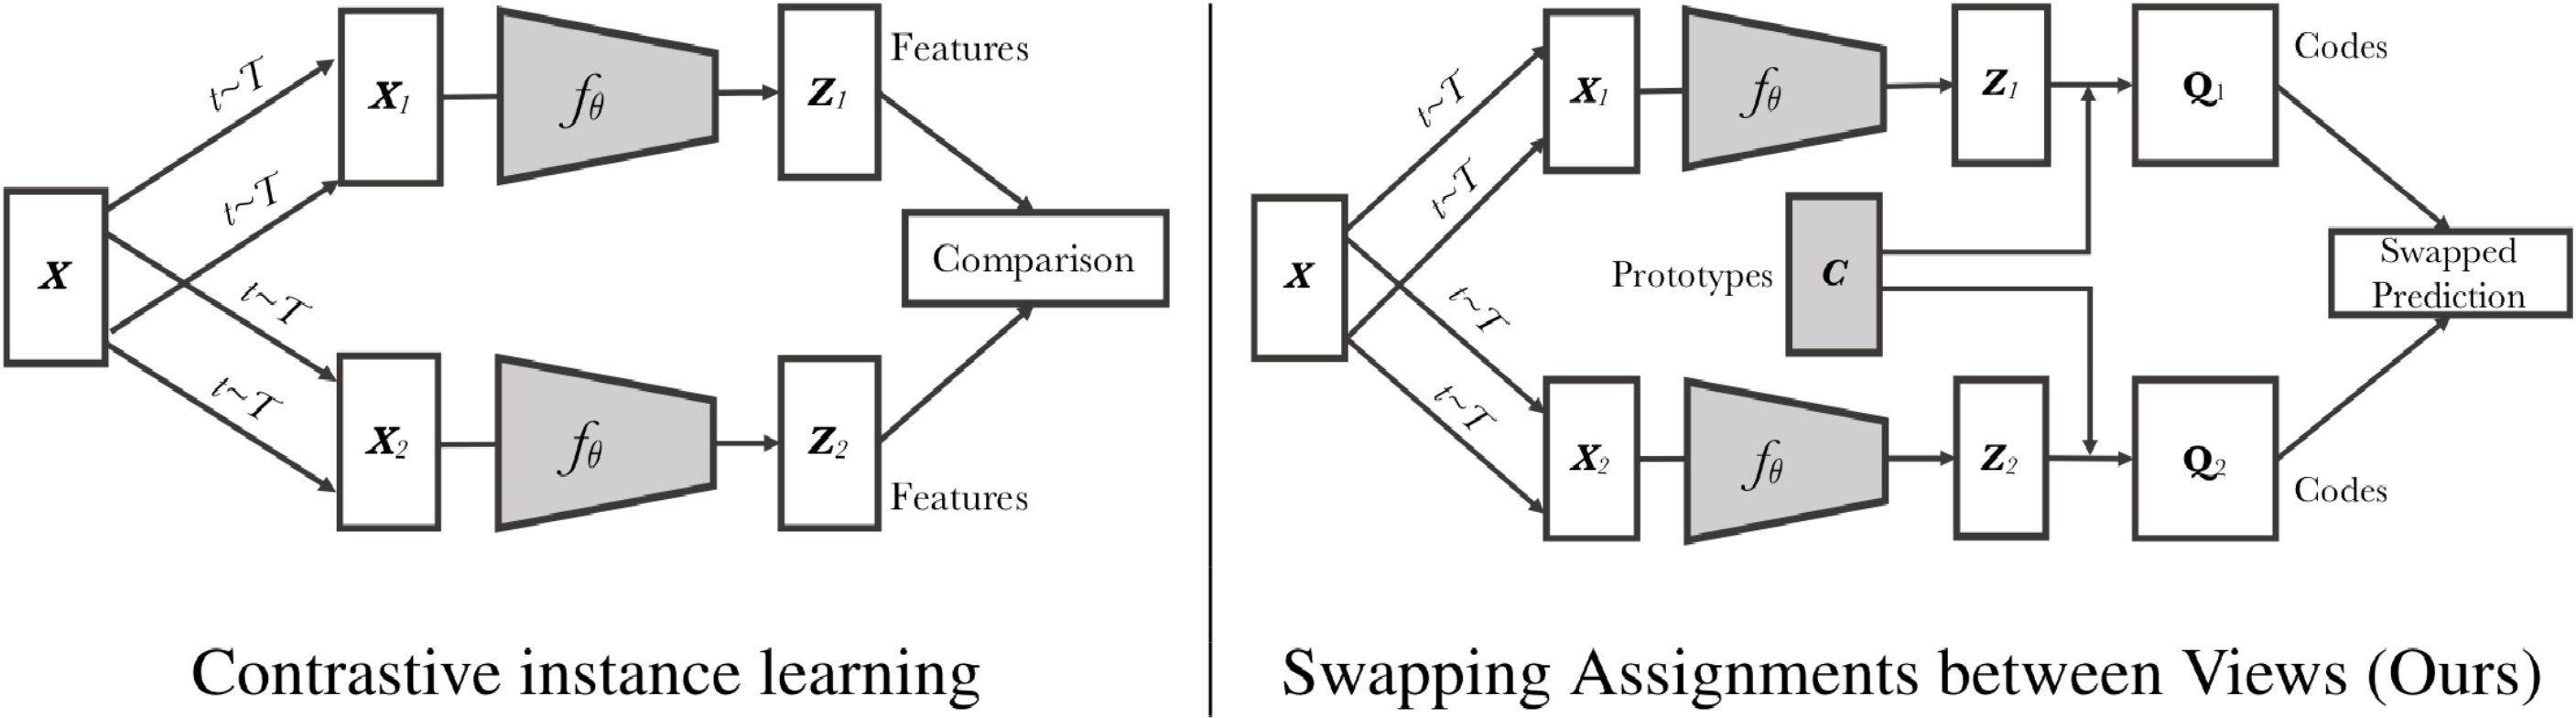
\includegraphics[width=300pt]{images/SwAV_vs_CL.png}
    \caption{Comparison of \ac{cl} and \ac{swav} from \citet{swav_2020}.
    \ac{cl} compares the augmented views directly while 
    \ac{swav} compares cluster assignments.
    Moreover, \ac{swav} computes the loss for an image and the cluster assignments of a positive augmentation 
    rather than its assignments and vice versa.}
    \label{fig:swav_vs_cl}
\end{figure}




% interesting approaches
%PCL
\subsubsection{\acl{pcl}}\label{subsec:PCL}

\citet{PCL_2021} use clustering in the feature space to optimize the sample's representation.
Each sample is associated with $M$ prototypes, which are obtained through $k_m$-means clustering across various values of $m$.
These prototypes, represented by cluster centroids, act as latent variables and are classified as positive samples. 
A contrastive loss is applied to ensure that the sample's embedding aligns closely with its assigned prototypes.
The so-called prototypical contrastive loss ProtoNCE is optimized using an \ac{em} algorithm 
as displayed in \autoref{fig:PCL_training}.

\begin{figure}[!htb] % h = here, t = top, b = bottom, p = page of floats
    \centering
    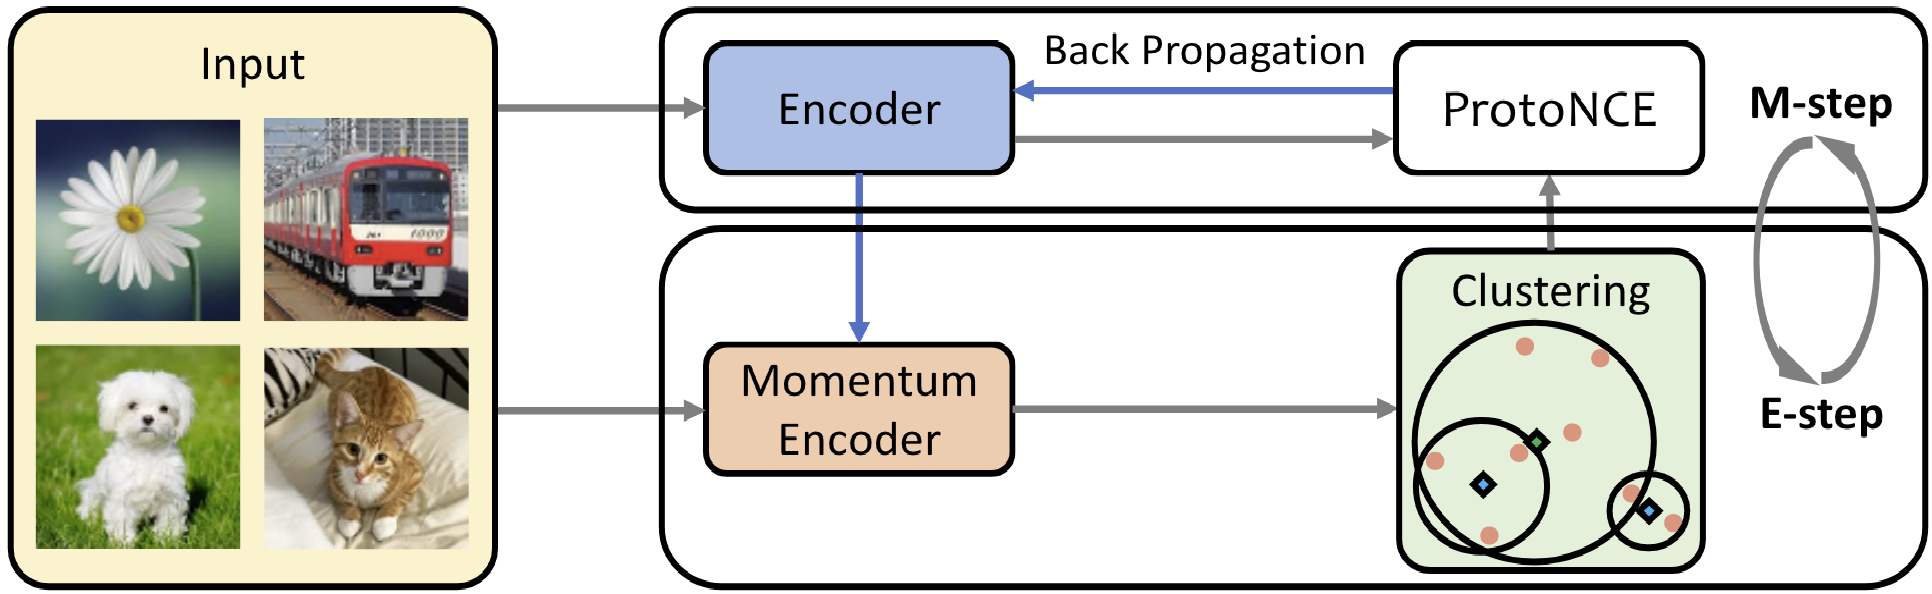
\includegraphics[width=360pt]{images/PCL_training.png}
    \caption{Illustration from \citet{PCL_2021}.
    The training process of the \ac{pcl} algorithm is demonstrated.
    $M$ $k_m$-means clusterings based on the feature space defined by the momentum encoder 
    are performed in the E-step.
    The prototypes $c^m_{\tilde{k}}$, $\tilde{k} \in [1, k_m]$, illustrated as green/ blue rectangles, 
    are the cluster centroids.
    The M-step updates the network parameters $\theta$ by optimizing the ProtoNCE loss.
    }
    \label{fig:PCL_training}
\end{figure}

% E-step: define k clusters & momentum encoder
$k$-means clustering is used to find the prototypes in the E-step.
The clustering is performed on the samples' embeddings obtained from the momentum encoder, 
whose parameters are a moving average of the main encoder's parameters and thus, smoother \citep{PCL_2021}.

% M-step
The M-step updates the network parameters $\theta$ by optimizing the ProtoNCE loss.
The minimization of the ProtoNCE loss is equivalent to maximizing the estimated log-likelihood.
The optimal parameters are those that map a sample close to its prototypes.
The result is obtained under the assumptions of a uniform prior over the cluster centroids, i.e. prototypes,
and an isotropic Gaussian distribution of the sample's embeddings around the prototypes.

% ProtoNCE loss
The ProtoNCE loss from \Eqref{eq:ProtoNCE} extends the InfoNCE from \Eqref{eq:InfoNCE} 
by not only enforcing similarity between the sample $z_i$ and 
one positive sample $z_i'$ while retaining dissimilarity to $r$ negative samples $z_j'$, 
but also considering its prototypes $c^m_s$. 
To enhance the stability of the results, $M$ clusterings are performed with varying numbers of clusters $k_m$. 
The use of different $k_m$ introduces varying levels of granularity among the prototypes, 
thereby encoding a hierarchical structure into the loss function.

\begin{equation}
    \mathcal{L}_{InfoNCE}= - \sum_{i=1}^{N}\log\frac{\exp \frac{z_i\cdot z_i'}{\tau}}{\sum_{j=0}^{r}\exp \frac{z_i\cdot z_j'}{\tau}}
    \label{eq:InfoNCE}
\end{equation}

\begin{equation}
    \mathcal{L}_{ProtoNCE}=\mathcal{L}_{InfoNCE} - \sum_{i=1}^{N} \frac{1}{M} \sum_{m=1}^{M} \log\frac{\exp \frac{z_i\cdot c_s^m}{\phi^m_s}}{\sum_{j=0}^{k_m}\exp \frac{z_i\cdot c_j^m}{\phi^m_j}}
    \label{eq:ProtoNCE}
\end{equation}




% Local Aggregation

\subsubsection{\acl{la}}\label{subsec:local_aggregation}

% s. unten: Hyperparameter prob- woher? k, H ist getestet, zumindest das Verhältnis, aber lambda wird aus anderer Arbeit übernommen -> keine Hyperparameter Suche

\citet{local_aggr_2019} optimize a low-dimensional feature space mapping by 
iteratively identifying close neighbours and updating the embedding function.
This soft clustering technique is called \ac{la}.

At each step during training of the embedding function $f_\theta: \mathcal{X} \rightarrow \mathcal{Z}$, 
two sets of neighbours are identified for each datapoint's embedding $z_i$ 
which are illustrated in \autoref{fig:la_bi_ci}.
The first set $C_i$ contains $z_i$'s close neighbours in the feature space, while
the second set $B_i$ contains $z_i$'s background neighbours.
$B_i$ is used as a means to judge distance and similarity, 
while $C_i$'s members should be embedded closer to $z_i$.
In other words, $C_i$ can be considered the set of positive samples while 
$B_i$ denotes the set of negative samples.
The level of \ac{la} $L(C_i,B_i | \theta, x_i)$ 
characterizes the relative level of closeness within $C_i$ compared to $B_i$.
$L(C_i,B_i | \theta, x_i)$ should be maximized.

The set $B_i$ consists of the $k$ nearest neighbours of $z_i$ in terms of cosine distance 
in the feature space.
$k$ is a hyperparameter and \citet{local_aggr_2019} set $k=4096$.
In order to construct $C_i$, 
first $H$ $k$-means clusterings are performed with sligthly different conditions.
Then, all of $z_i$'s clusters are united to form $C_i$.
$H$ and $k$ are hyperparameters.
\citet{local_aggr_2019} find that more clusterings, i.e. higher $H$, lead to isotropic clusters since outliers which arise from random processes are averaged out.
If $H$ is too high compared to the number of clusters $k$, the performance decreases.
They state that $H=3, k=10000$ and $H=10, k=30000$ are better values than $H=10, k=10000$ 
in terms of ResNet-18 nearest neighbour validation performance.

Finally, the level of \ac{la} $L(C_i,B_i | \theta, x_i)$ is defined as the negative log-likelihood 
of the feature space representation $z_i$ of $x_i$ being in $C_i$ given $B_i$, 
i.e., being recognized as a close neighbour given being recognized as a background neighbour.
The loss to minimize is $\mathcal{L} = L(C_i,B_i | \theta, x_i) + \lambda \left\| \theta \right\|^2$.
\citet{local_aggr_2019} choose to rely on hyperparameter settings from another work rather than conducting a hyperparameter search.

\begin{figure}[!htb] % h = here, t = top, b = bottom, p = page of floats
    \centering
    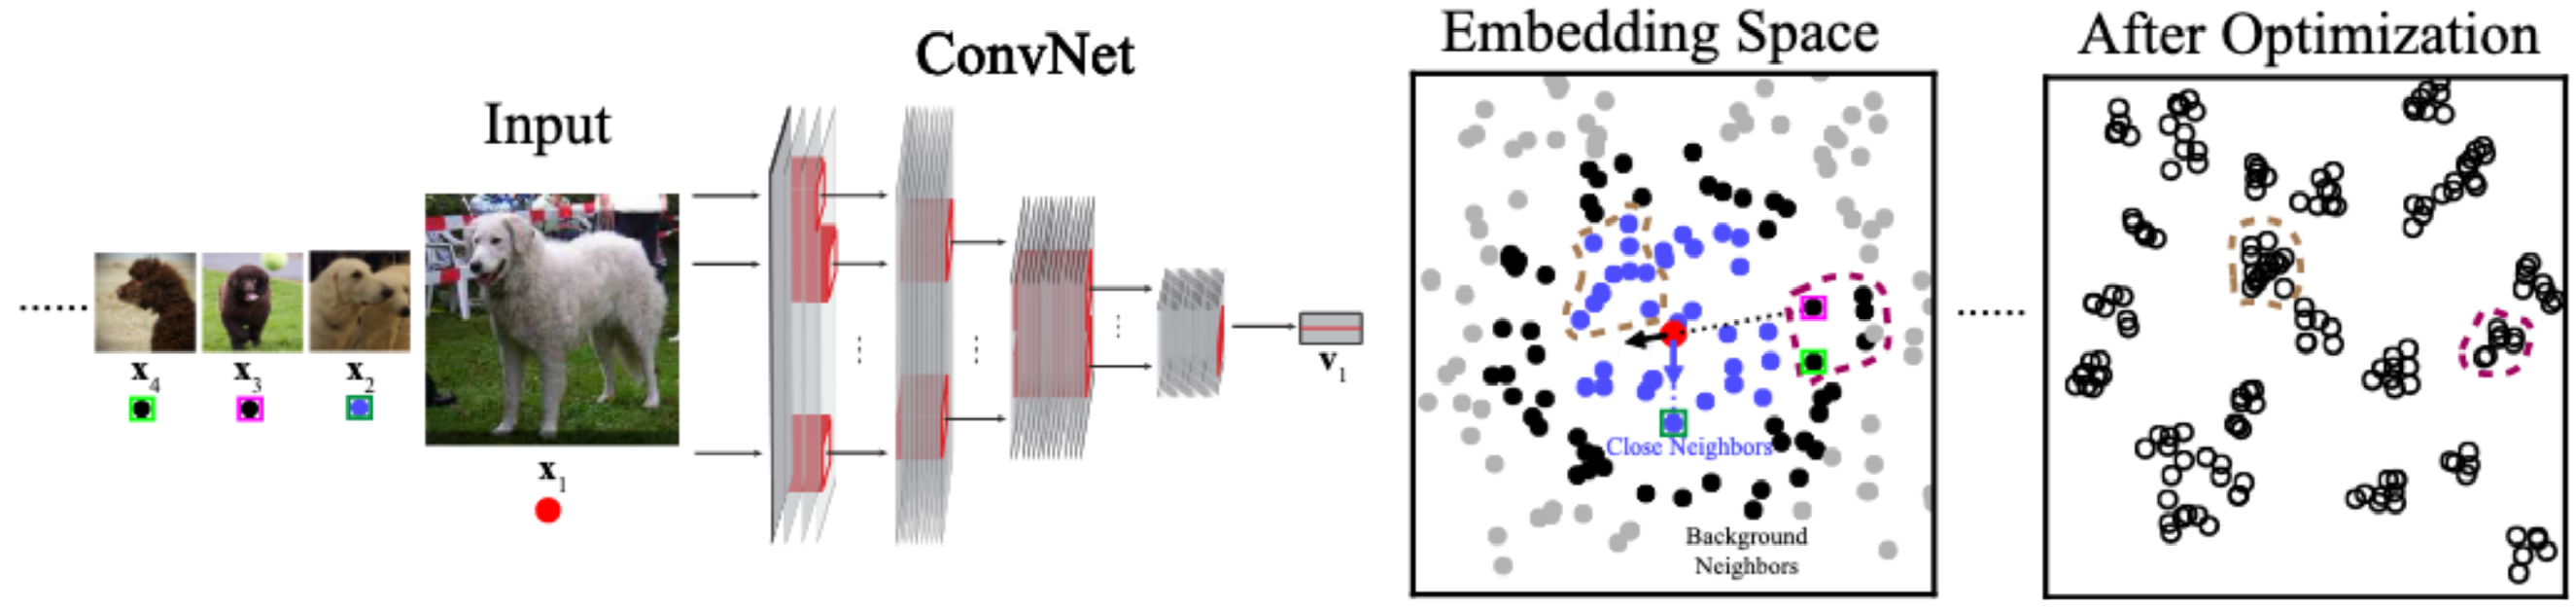
\includegraphics[width=360pt]{images/la_neighbourhoods.png}
    \caption{Illustration from \citet{local_aggr_2019}.
    A \ac{cnn} produces the feature space embedding $z_i = f_\theta(x_i)$.
    The embeddings are displayed as points in the feature space.
    The red point is the anchor $z_i$, 
    whereas blue points are close neighbours $C_i$ and
    black points are background neighbours $B_i$.
    The arrows denote influences between the neighbours.}
    \label{fig:la_bi_ci}
\end{figure}

% Mining on manifolds
\subsubsection{Mining on manifolds}\label{subsec:mining_manifolds}


% sparse usage of hard pairs inspired by SVMs

% purpose
According to \citet{mining_manifolds_2018}, the initial representation of the data is obtained by e.g. a pre-trained \ac{cnn}.
Hard pair mining is performed in order to fine-tune the network.

% idea of positive and negative samples
For fine-tuning, a combination of different definitions of proximity induces mining 
for hard positives and negatives as displayed in \autoref{fig:mining_manifolds_vis}.
Given an anchor, samples that reside on the same manifold but 
are not proximate in terms of Euclidean distance are considered hard positive samples.
These positive samples should be embedded closer to the anchor in the Euclidean space.
Conversely, hard negative samples are those that are spatially proximate in Euclidean space 
yet lie on different manifolds.
These samples should be embedded further away from the anchor in the Euclidean space.
%The hard samples are mined from an unordered set of \textit{relevant} samples.

% different neighbourhoods & hard samples
The authors denote the set of the $k$ nearest Euclidean neighbours $NN^e_k$ and 
the $k$ nearest manifold neighbours $NN^m_k$.
The hard positives are defined as $NN^m_k \textbackslash NN^e_k$. 
The pool $NN^m_k$ is ordered by descending manifold similarity to the anchor
to ensure that high-confidence samples are chosen first.
$k$ controls the diversity of the hard positives.
The larger $k$ is, the more diverse, i.e. hard, the hard positives are. 
The pool of hard negatives is defined as $NN^e_k \textbackslash NN^m_k$.
$NN^e_k$ is ordered by descending Euclidean distance to the anchor to keep the hardest samples.

% visualization of hard samples
\begin{figure}[!htb]% h = here, t = top, b = bottom, p = page of floats
    \centering
    \subfloat[\centering $k$ nearest Euclidean neighbour $NN^e_k$ (orange).]
    {{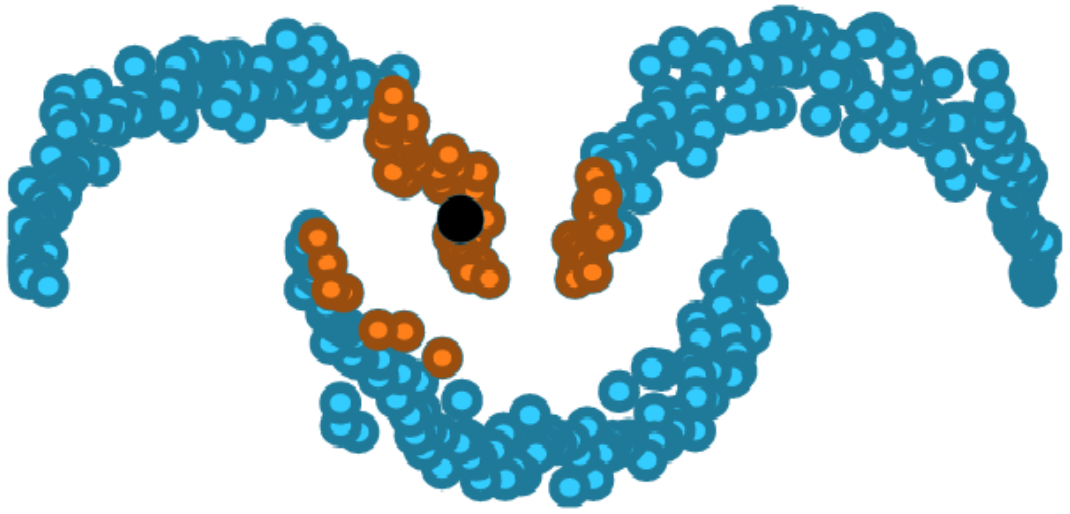
\includegraphics[width=5cm]{images/euclidean_NN.png} }}%
    \qquad
    \subfloat[\centering $k$ nearest manifold neighbour $NN^m_k$ (purple).]
    {{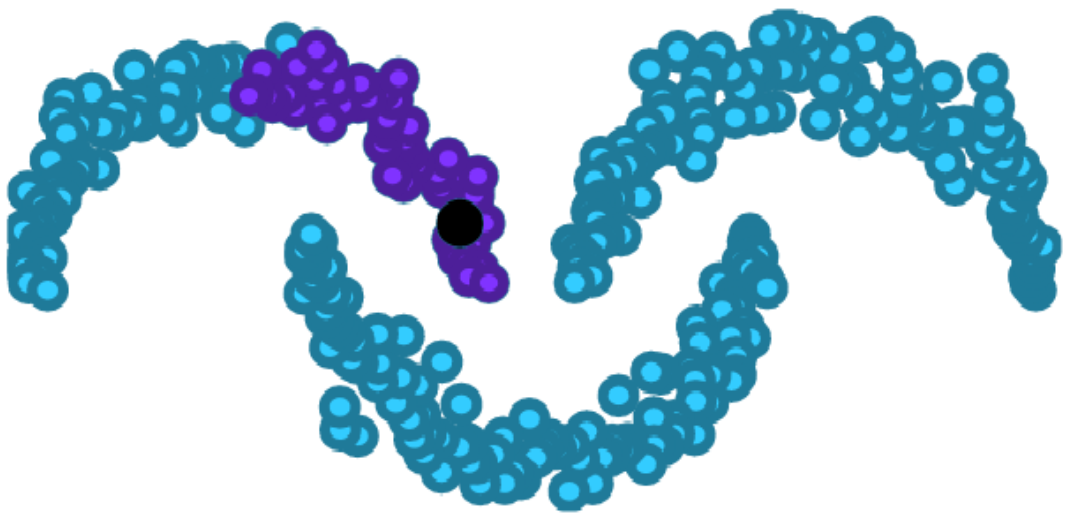
\includegraphics[width=5cm]{images/manifold_NN.png} }}%
    \qquad
    \subfloat[\centering Hard positives $NN^m_k \textbackslash NN^e_k$(green).]
    {{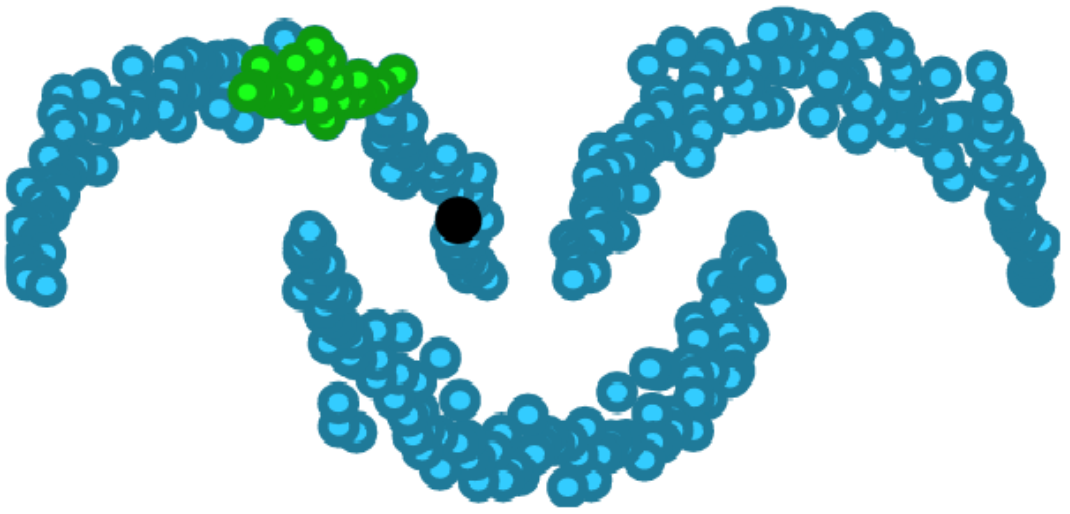
\includegraphics[width=5cm]{images/hard_positives_manifold.png} }}%
    \qquad
    \subfloat[\centering Hard negatives $NN^e_k \textbackslash NN^m_k$(red).]
    {{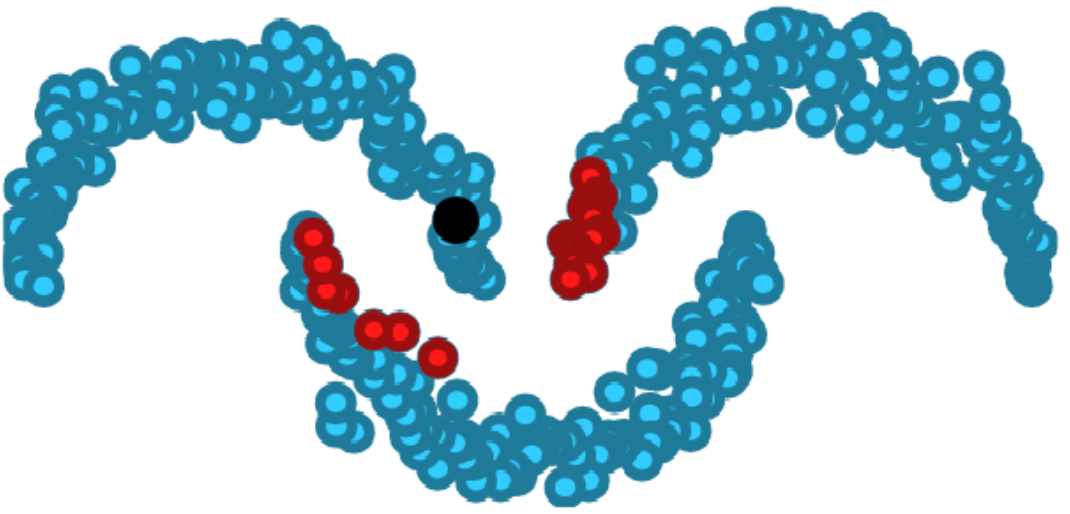
\includegraphics[width=5cm]{images/hard_negatives_euclidean.png} }}%

    \caption{Visualization of different proximity definitions, 
    the hard negatives and positives from \citet{mining_manifolds_2018}.
    The anchor is the black point.}%
    \label{fig:mining_manifolds_vis}%
\end{figure}


% manifolds via random walk n nearest neighbour graph
\citet{mining_manifolds_2018} propose a method where the manifold is estimated by mode-seeking, i.e. a random walk process, 
on the Euclidean nearest neighbour graph induced by the Euclidean similarity function $s_e$.
The graph is undirected, weighted and represented by a sparse symmetric adjacency matrix.
The adjacency matrix is constructed from the reciprocal $k$ nearest neighbours of each sample, 
where two points are considered reciprocal if each belongs to the $k$ nearest neighbours of the other. 
To reduce the negative impact of outliers, only reciprocal nearest neighbours are incorporated \citep{diffusion_2017,mining_manifolds_2018,fast_2018}.
The weighted adjacency matrix entries $a_{ij}$ defined in \Eqref{eq:mining_manifolds_adjacency_matrix} from \citet{mining_manifolds_2018} 
are calculated via the Euclidean distance between the samples if both nodes are in each other's nearest neighbourhood.
Diagonal entries are set to zero \citep{mining_manifolds_2018,fast_2018}.
%They admit that assessing the manifold similarity poses additional computational and memory requirements.
The manifold is computed once at the beginning \citep{mining_manifolds_2018}.

\begin{equation}
    a_{ij} = \begin{cases}
        s_e(y_i,y_j), & \text{if } y_i \in NN^e_k(y_j)\wedge y_j \in NN^e_k(y_i)\\
        0, & \text{otherwise}\\
      \end{cases}     
    \label{eq:mining_manifolds_adjacency_matrix}
\end{equation}


% mode seeking
% The manifold representation is obtained via mode-seeking as described in \citet{mode_seeking_2012}.
% The nearest neighbour network consists of samples as nodes and is weighted by the Euclidean distance 
% if both samples are in each other's $k$ nearest neighbourhood \citet{mode_seeking_2012,mining_manifolds_2018}.

% authority modes
While traditional mode-seeking relies on metric features, such as distances, mode-seeking on graphs 
uses the concept of random walks instead \citep{mode_seeking_2012}.
A random walk, i.e. a linear combination of the identity matrix and a scaled version of the adjacency matrix, is simulated multiple times on the graph.
\citet{mode_seeking_2012} define the so-called authority modes on a graph 
as the most frequently visited nodes by random walks among their local neighbours.
They correspond to the local maxima of the underlying probability distribution of random walks over the graph.
% selection of anchors
Since the anchors should be diverse and relevant, they are chosen to be the authority modes \citep{mining_manifolds_2018}.

% authority score
Inspired by PageRank, the possibility of random jumps is included in order to ensure convergence to a stationary distribution. 
The probability of visiting a node is denoted by the authority score $\pi$ 
which is defined in \Eqref{eq:authority_score} from \citet{mode_seeking_2012} 
where $p(i,j)$ are the entries of the Markov transition matrix $P$.
$\pi(j)$ takes into account the probability of visiting a node $j$ from a node $i$ and 
the probability of a random jump from one of the nodes chosen uniformly at random.
\citet{mode_seeking_2012} set $\alpha$ to $0.9$. 
The authority score $\pi$ can be computed by, for instance, the power method \citep{mode_seeking_2012,PageRank_2004}.

\begin{equation}
    \pi(j) = \alpha \sum_{i \in \mathcal{V}}^{}  \pi(i)p(i,j) + (1-\alpha)\frac{1}{N} , \text{ where } p(i,j) = \frac{a_{ij} }{\sum_{k \in \mathcal{V}}^{}a_{ik} } 
    \label{eq:authority_score}
\end{equation}

% local neighbours on the manifold: node relevancy 
\citet{mode_seeking_2012} define node relevancy $\Psi(s,t)$ via \Eqref{eq:node_relevancy} where $d(s)$ denotes the out-degree of a node.
To incorporate the reachability of a node, the probability of reaching node $t$ from node $s$ in $k$ steps $p_k(s,t)$ is 
defined via the $k_{th}$ power of the Markov transition matrix $P$.
To support similar authority scores between neighbouring nodes, the exponential term including a weighting factor $\gamma$ is included.
$\Psi(s,t)$ is not symmetric and depends on the random walk step $k$.
The authors propose to use the node relevancy $\Psi(s,t)$ for a node $s$ to determine the manifold neighbours $N_\varepsilon^m(s)$ for $s$ 
via the usage of a threshold $\varepsilon$: 
$N_\varepsilon^m(s) =  \left\{ t \in \mathcal{V} | \Psi(s,t) > \varepsilon \right\} \cup \left\{ s \right\}$ \citep{mode_seeking_2012}.

\begin{equation}
    \Psi(s,t) = d(s) p_k(s,t) \exp(-\gamma \left\{  \pi(t) - \pi(s)  \right\}^2)\text{, where } d(s) = \sum_{j\in \mathcal{V}}^{}a_{sj}
    \label{eq:node_relevancy}
\end{equation}

% AAS
They propose the \ac{aas} as a nonparametric estimator of the authority modes.
A node $s$ is shifted to node $\mathcal{A}(s)$ calculated in \Eqref{eq:authority_ascent_shift}. 
This formula chooses the local neighbour $t$ of $s$ that maximizes the difference of the authority scores $\pi$.
The authors argue that the \ac{aas} is finite and converges since the graph is finite.
When \ac{aas} is completed, manifolds are represented as clusters.
% examples
Resulting hard positives and negatives are displayed in \autoref{fig:manifold_mining_qualitative_analysis} and \autoref{fig:manifold_mining_examples}.

\begin{equation}
    \mathcal{A}(s) = \underset{t \in \mathcal{N_\varepsilon}(s)}{\text{argmax}} \left\{ p_k(s,t)\left[ \pi(t)-\pi(s) \right] \right\}
    \label{eq:authority_ascent_shift}
\end{equation}

% inlier and outlier
% Inliers on the manifold reside in large clusters while outliers are isolated in small groups since they do not have enough relevancy with inliers \citet{mode_seeking_2012}.
% Hence, outlier clusters can be identified by low sums of authority values.


\begin{figure}[!htb] % h = here, t = top, b = bottom, p = page of floats
    \centering
    \includegraphics[width=300pt]{images/mining_manifold_qualitative_analysis.png}
    \caption{Illustration of CUB200-2011 from \citet{mining_manifolds_2018}.
    The anchor is denoted $x^r$.
    A selection of hard positives from $P^+(x^r)$ is compared to the 
    baseline approach that samples from the closest neighbours to $x^r$ in 
    terms of Euclidean distance.
    Analogously, a selection of hard negatives from $P^-(x^r)$ 
    is compared to the baseline $X \textbackslash NN^e_3$, 
    i.e. sampling from the set that contains all samples but the three closest ones in 
    terms of Euclidean distance.
    The borders of the images denote the ground-truth class, i.e. if bird species is the same.
    Green borders indicate that the image belongs to the same class as the anchor, 
    while red borders signify images from a different class.
    It becomes apparent that the sampled hard positives consist of fewer false positives 
    than the baseline.
    }
    \label{fig:manifold_mining_qualitative_analysis}
\end{figure}

\begin{figure}[!htb] % h = here, t = top, b = bottom, p = page of floats
    \centering
    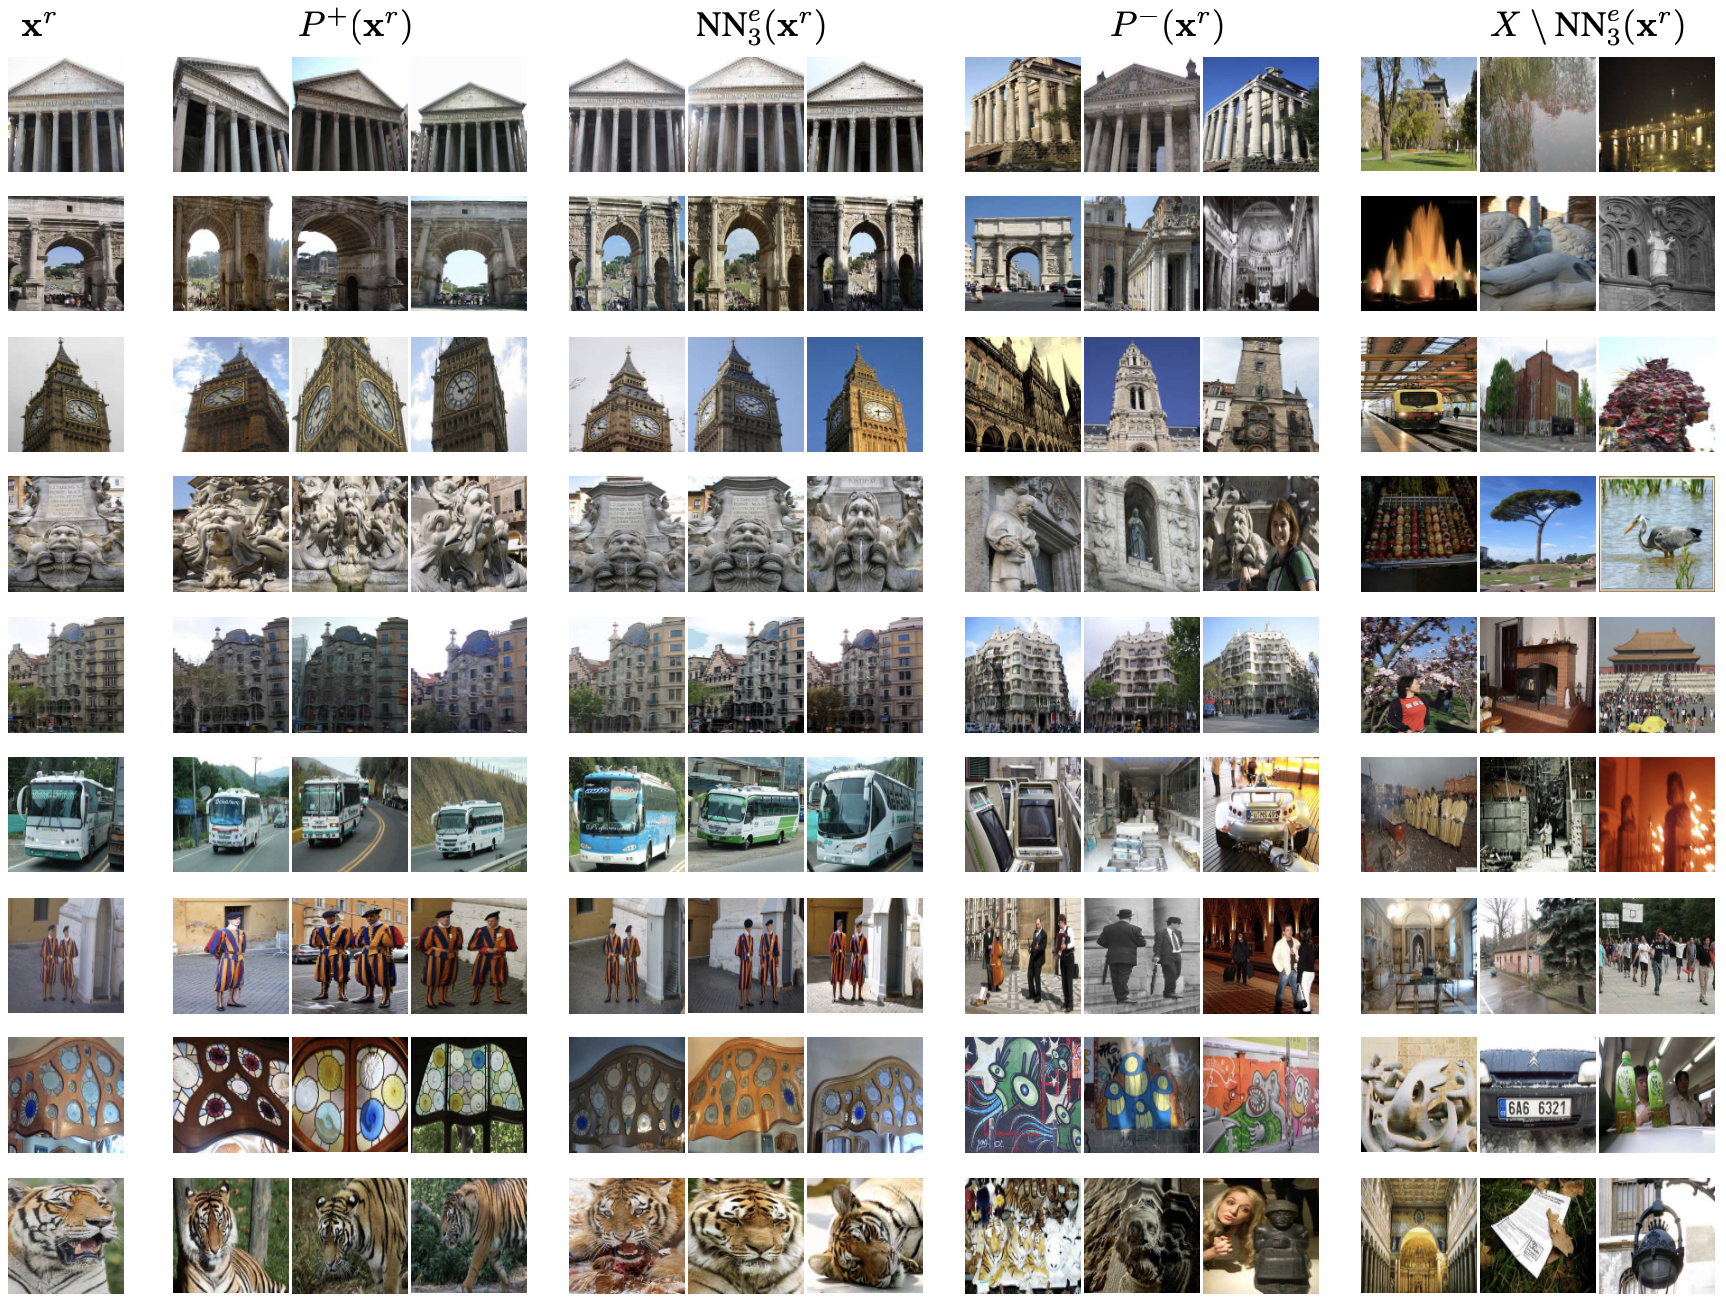
\includegraphics[width=360pt]{images/mining_manifold_examples.png}
    \caption{Illustration Oxford5k and Paris6k images crawled from Flickr from \citet{mining_manifolds_2018}.
    The dataset contains multiple images for each landmark building, i.e. class \citep{manifold_dataset}.
    The anchor is denoted $x^r$.
    A selection of hard positives from $P^+(x^r)$ is compared to the 
    baseline approach that samples from the closest neighbours to $x^r$ in 
    terms of Euclidean distance.
    Analogously, a selection of hard negatives from $P^-(x^r)$ 
    is compared to the baseline $X \textbackslash NN^e_3$, 
    i.e. sampling from the set that contains all samples but the three closest ones in 
    terms of Euclidean distance.
    It becomes apparent that the hard negatives display visually similar but 
    semantically different images to the anchor. % good
    }
    \label{fig:manifold_mining_examples}
\end{figure}

% loss functions
The authors propose multiple loss functions to train the model.
They, for instance, apply the contrastive loss $l_c(x^r, x^+, x^-)= \left\| x^r - x^+ \right\|^2 + \left[ m - \left\| x^r - x^- \right\| \right]^2$, 
the triplet loss $l_t(x^r, x^+, x^-)= \left[ m +  \left\| x^r - x^+ \right\| ^2 - \left\| x^r - x^- \right\| \right]^2$, 
and weighted versions of both contrastive and triplet loss, where the loss is multiplied by the manifold similarity of anchor and positive sample \citep{mining_manifolds_2018}.
$m$ is a margin parameter and $x^r$ is the representation of the anchor.

% effect of temperature on contrastive learning loss function & embedding space

The parameter $\tau$ is called temperature.
\citet{wang_understanding_2021} have carried out an exhaustive study on the impact of temperature on the loss function of \ac{cl}.
They found that the contrastive loss function optimizes hard samples by penalizing them according to their hardness.
Small temperatures $\tau$ penalize very hard negative samples, i.e. similar to the anchor.
Hence, the samples' representations are pushed further apart and thus, the embedding space becomes more uniformly distributed.
For $\tau \rightarrow \infty$, the loss function's hardness-aware property disappears and hard negatives are not penalized anymore.
However, when $\tau$ is too small, the embedding spaces' semantic structure deteriorates.


\begin{figure}%
    \centering
    \subfloat[\centering For small values of $\tau$, similar samples, i.e. x-axis values close to $1.0$, receive high penalties.
    If $\tau$ is too small, only the closest one or two points are penalized and thus, the performance deteriorates.
    As $\tau \rightarrow 1$, the magnitude of the penalty is similar for all negative samples.]
    {{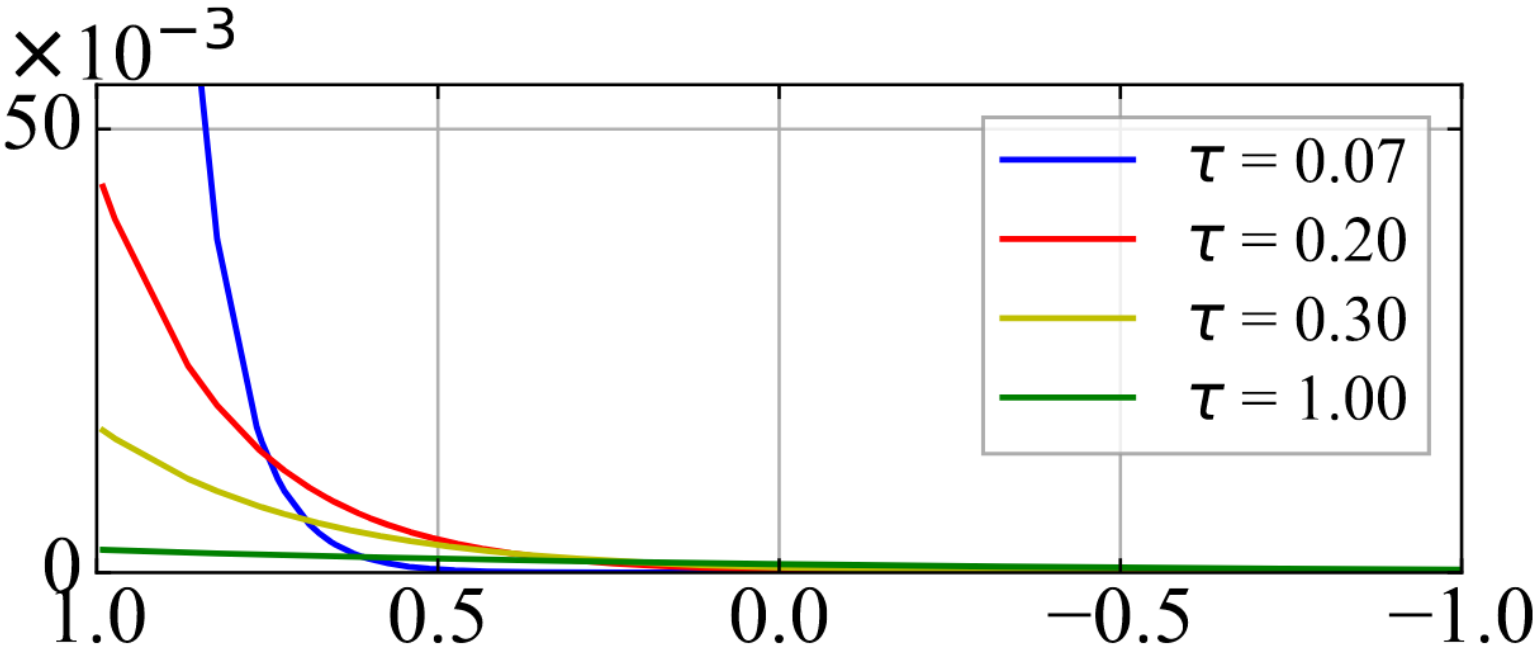
\includegraphics[width=6cm]{images/gradient_ratio_dep_on_temperature.png} }}%
    \qquad
    \subfloat[\centering Visualization of embedding space for different $\tau$.
    Small values of $\tau$ lead to a more uniform distribution of the embedding space, 
    because similar samples are repelled.]
    {{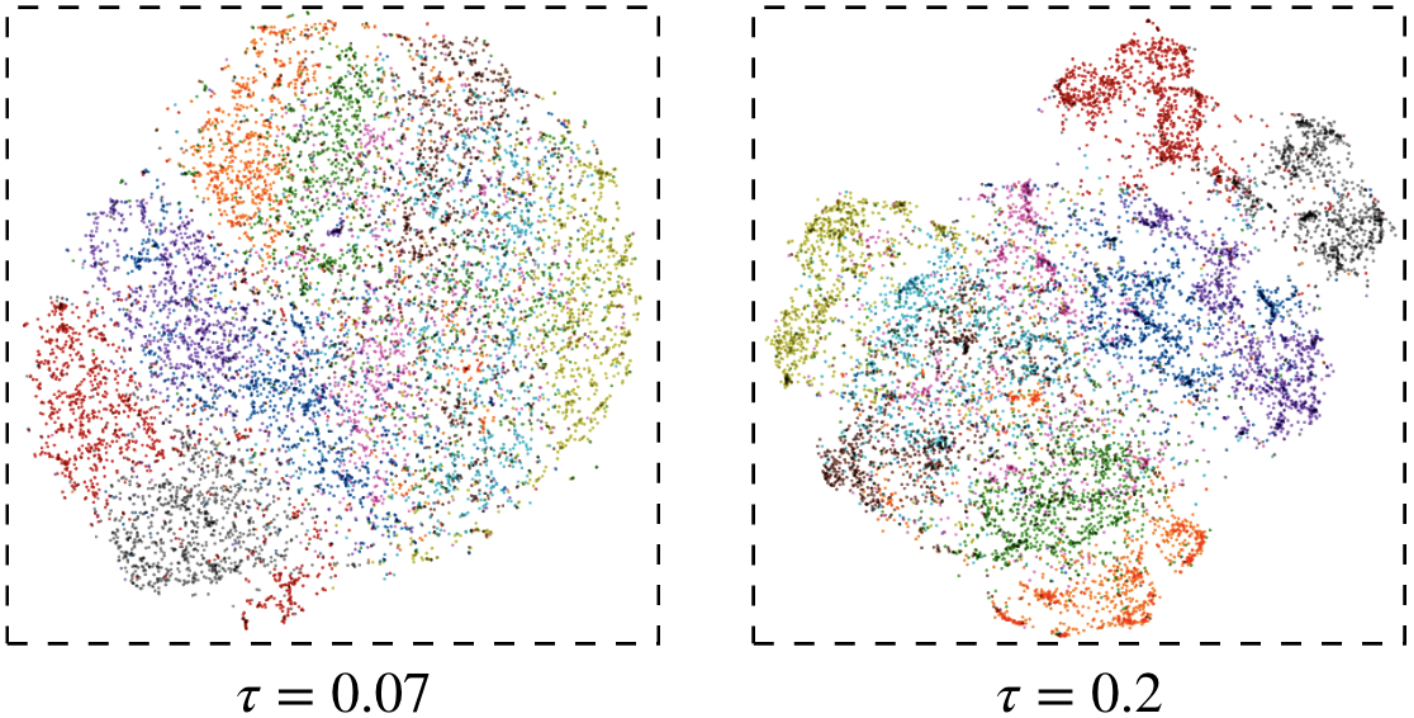
\includegraphics[width=4cm]{images/tsne_dep_on_temperature.png} }}%
    \caption{Illustrations from \citet{wang_understanding_2021}.}%
    \label{fig:temperature}%
\end{figure}

% \begin{figure}[h] % h = here, t = top, b = bottom, p = page of floats
%     \centering
%     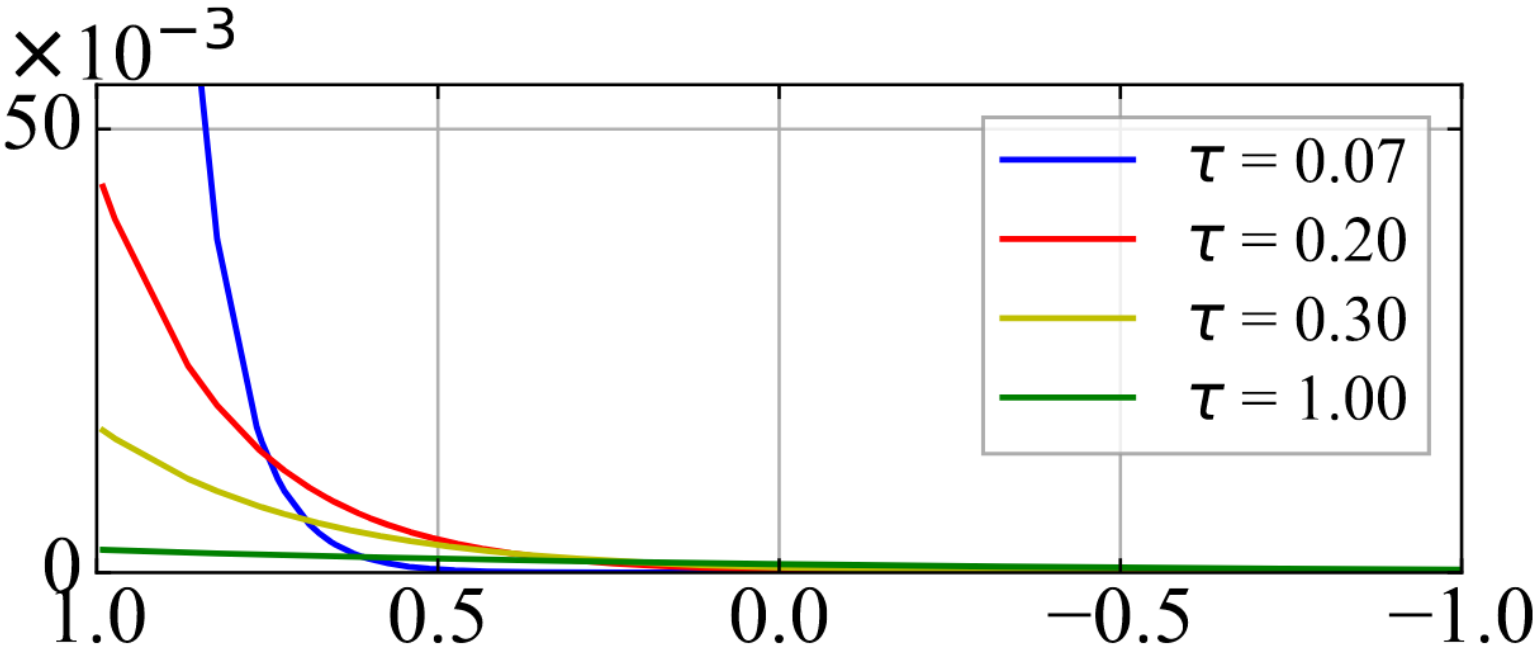
\includegraphics[width=360pt]{images/gradient_ratio_dep_on_temperature.png}
%     \caption{Illustration from \citet{wang_understanding_2021}.
%     For small values of $\tau$, similar samples, i.e. x-axis values close to $1.0$, receive high penalties.
%     If $\tau$ is too small, only the closest one or two points are penalized and thus, the performance deteriorates.
%     As $\tau \rightarrow 1$, the magnitude of penalty is similar for all negative samples.
%     }
%     \label{fig:gradient_ratio_dep_on_temperature}
% \end{figure}

% \begin{figure}[h] % h = here, t = top, b = bottom, p = page of floats
%     \centering
%     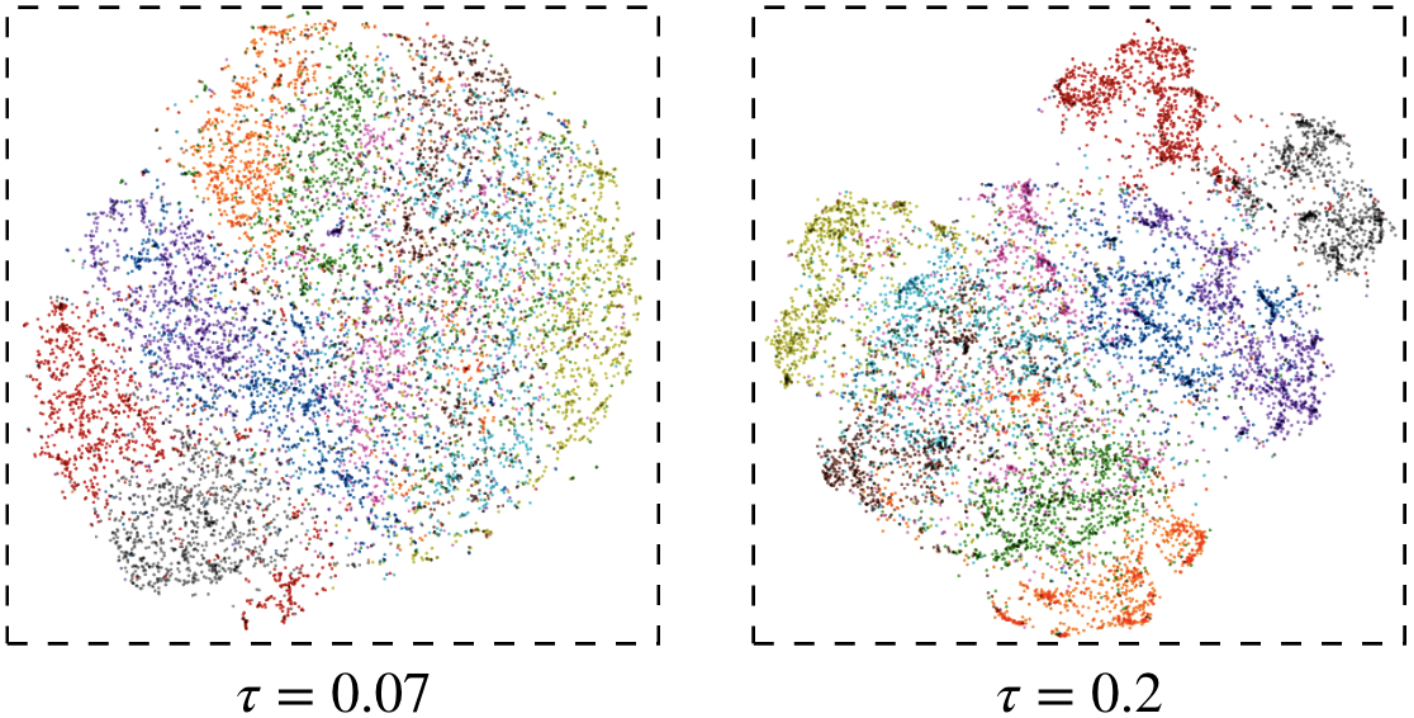
\includegraphics[width=360pt]{images/tsne_dep_on_temperature.png}
%     \caption{Visualization of embedding space for different $\tau$ from \citet{wang_understanding_2021}.
%     Small values of $\tau$ lead to a more uniform distribution of the embedding space, 
%     because similar samples are repelled.
%     }
%     \label{fig:tsne_dep_on_temperature}
% \end{figure}

% graph models
\citet{grape_2024} have worked on a \ac{cl} approach on graphs called \ac{grape}.
According to \citeauthor{grape_2024}, small values of $\tau$ lead to strong repulsive forces on neighboring samples.
Larger values of $\tau$, on the other hand, exert weaker repulse forces. % info for eg. PCL

% memory bank
\subsection{\acl{mochi}}\label{subsec:MoCHi}

\citet{mochi_2020} claim that most approaches to sampling negatives rely on 
time-consuming updates of a memory bank or big batches to achieve good performance.
They propose \ac{mochi}, a method that computes samples online claiming without any computational overhead.

% memory bank
They use a memory bank $Q$ of size $| Q | = K$ to store negative samples.
There are different ways to choose $K$ by either saving the whole dataset, a queue of the last batches,
or all images in the current batch.

% definition of MoCHi
The definition of \ac{mochi}($N, s, s'$) is as follows:
\begin{enumerate}
    \item $N$: Number of negative samples from the memory bank to consider during negative mining.
    \item $s$: Number of samples to generate with approach 1.
    \item $s'$: Number of samples to generate with approach 2.
\end{enumerate}
For both approaches to generating negative samples, the authors use the same memory bank $Q$.
Given a fixed anchor, firstly, $Q$ is ordered in descending similarity to the anchor representation    
in the feature space producing $\tilde{Q}$.
The similarity between $n_j \in \tilde{Q}$ and the query $q$ is calculated via 
a scaled dot product of both samples.
Secondly, all but the first, i.e. most similar, $N$ samples are discarded from $\tilde{Q}$.
% first approach
The first approach proposed by \citeauthor{mochi_2020}, chooses two random samples $n_i, n_j \in \tilde{Q}$ 
and a mixing coefficient $\alpha_k \in (0,1)$, 
to generate the new sample as a linear combination of the existing hard negative samples 
as described in \eqref{eq:mochi_appr1}.

\begin{equation}
    h_k = \frac{\tilde{h_k}}{\left\| \tilde{h_k}  \right\|}; \tilde{h_k} = \alpha_k n_i + (1-\alpha_k)n_j
    \label{eq:mochi_appr1}
\end{equation}

% second approach
The second approach generates new samples by using the anchor representation $q$ 
and a random sample $n_j \in \tilde{Q}$ to generate the new sample as described in \eqref{eq:mochi_appr2}.
The mixing coefficient $\beta_k \in (0,0.5)$ is used to balance the influence of the anchor 
and the hard negative sample.
By limiting the influence of the anchor, the authors enforce a stronger influence of the negative sample.
This approach is considered to produce even harder negative samples than the first approach.

\begin{equation}
    h_k' = \frac{\tilde{h_k'}}{\left\| \tilde{h_k'}  \right\|}; \tilde{h_k'} = \beta q + (1-\beta_k)n_j
    \label{eq:mochi_appr2}
\end{equation}

% update of memory bank
Using \eqref{eq:mochi_appr1} and \eqref{eq:mochi_appr2}, 
$s$ and $s'$ hard negative samples are generated respectively.
Afterward, the similarity of each generated sample $h_k$ (or $h_k'$ respectively) 
to the anchor $q$ is calculated via $\frac{q^T h_k}{\tau}$.
This similarity is used to update the memory bank $\tilde{Q}$ 
by inserting the new sample.

% loss functions
There are two loss functions proposed by \citet{mochi_2020} to train the model.
Firstly, the alignment loss is used to determine 
the absolute distance between representations with the same class label.
Secondly, the uniformity loss is used to determine 
the distribution of representations on the hyperphere.
It is calculated via the logarithm of the average pairwise Gaussian potential between all embeddings.

% s, s' effect
\citet{mochi_2020} conducted experiments to investigate the effect of the parameters $s, s'$.
They present metrics such as average precision and accuracy for different ratios of $s$ and $s'$ 
for object detection and image segmentation tasks on COCO as well as 
linear classification on ImageNet-1K and object detection on PASCAL VOC.
Generally, the scores differ only in magnitudes of $1 \%$.
Additionally, the authors state that for $s > 0, s' = 0$ the model learns faster but achieves similar performance to the baseline, i.e. the model without \ac{mochi}.


% modifications
The authors listed modifications to \ac{mochi} that lead to inferior performance.
They tried to define the mixing coefficient via the similarity of the hard negative samples 
to the anchor. % how negative the sample is 
Moreover, they introduced non-uniformity when sampling $n_i, n_j$ from $\tilde{Q}$ by defining a 
probability distribution over similarities to the query. % too hard samples
Alternatively, they proposed omitting the parameters $s, s'$ and 
sampling hard negatives using alternately approaches 1 and 2 until $N\%$ of the top samples in 
$\tilde{Q}$ correspond to synthesized samples.

% scheme 2 from ProGCL: ProGCL-mix (MoCHi)
\begin{equation}
    \tilde{h_k} =  \alpha_k \cdot n_i + (1-\alpha_k) \cdot  n_j, \text{ where } \alpha_k = \frac{p(n_i \text{ is } TP)}{p(n_i \text{ is } TP) + p(n_j \text{ is } TP)}
    \label{eq:progcl_mix}
\end{equation}

The researches that introduced \progcl{} (\autoref{subsec:graph_distribution}) in \citet{progcl_2022} 
present an extension of the hard mining strategy \ac{mochi}.% introduced in \autoref{subsec:MoCHi}.
They claim, that a high portion of the negative samples generated by \ac{mochi} are \acp{fn}.
They therefore propose to weigh the selected negative samples for mixing 
according to their relative probability of being a \ac{tn} as displayed in \eqref{eq:progcl_mix}.

% others
\subsection{Curricular weighting}\label{subsec:curricular_weighting}

\citet{curricular_weighting_2024} propose a weighting scheme for the negative samples 
in the context of \ac{cl}, which emulates human learning.
Initially, the model is trained on easy negative samples and gradually prioritizes harder negative samples 
as displayed in \autoref{fig:curriculum_learning_samples}.
Therefore, the weight of hard negative samples is increased over time according to the model performance.
Furthermore, the authors introduce a $\mathcal{L}_2$ regularization term to mitigate the influence of \acp{fn}.

\begin{figure}[h] % h = here, t = top, b = bottom, p = page of floats
    \centering
    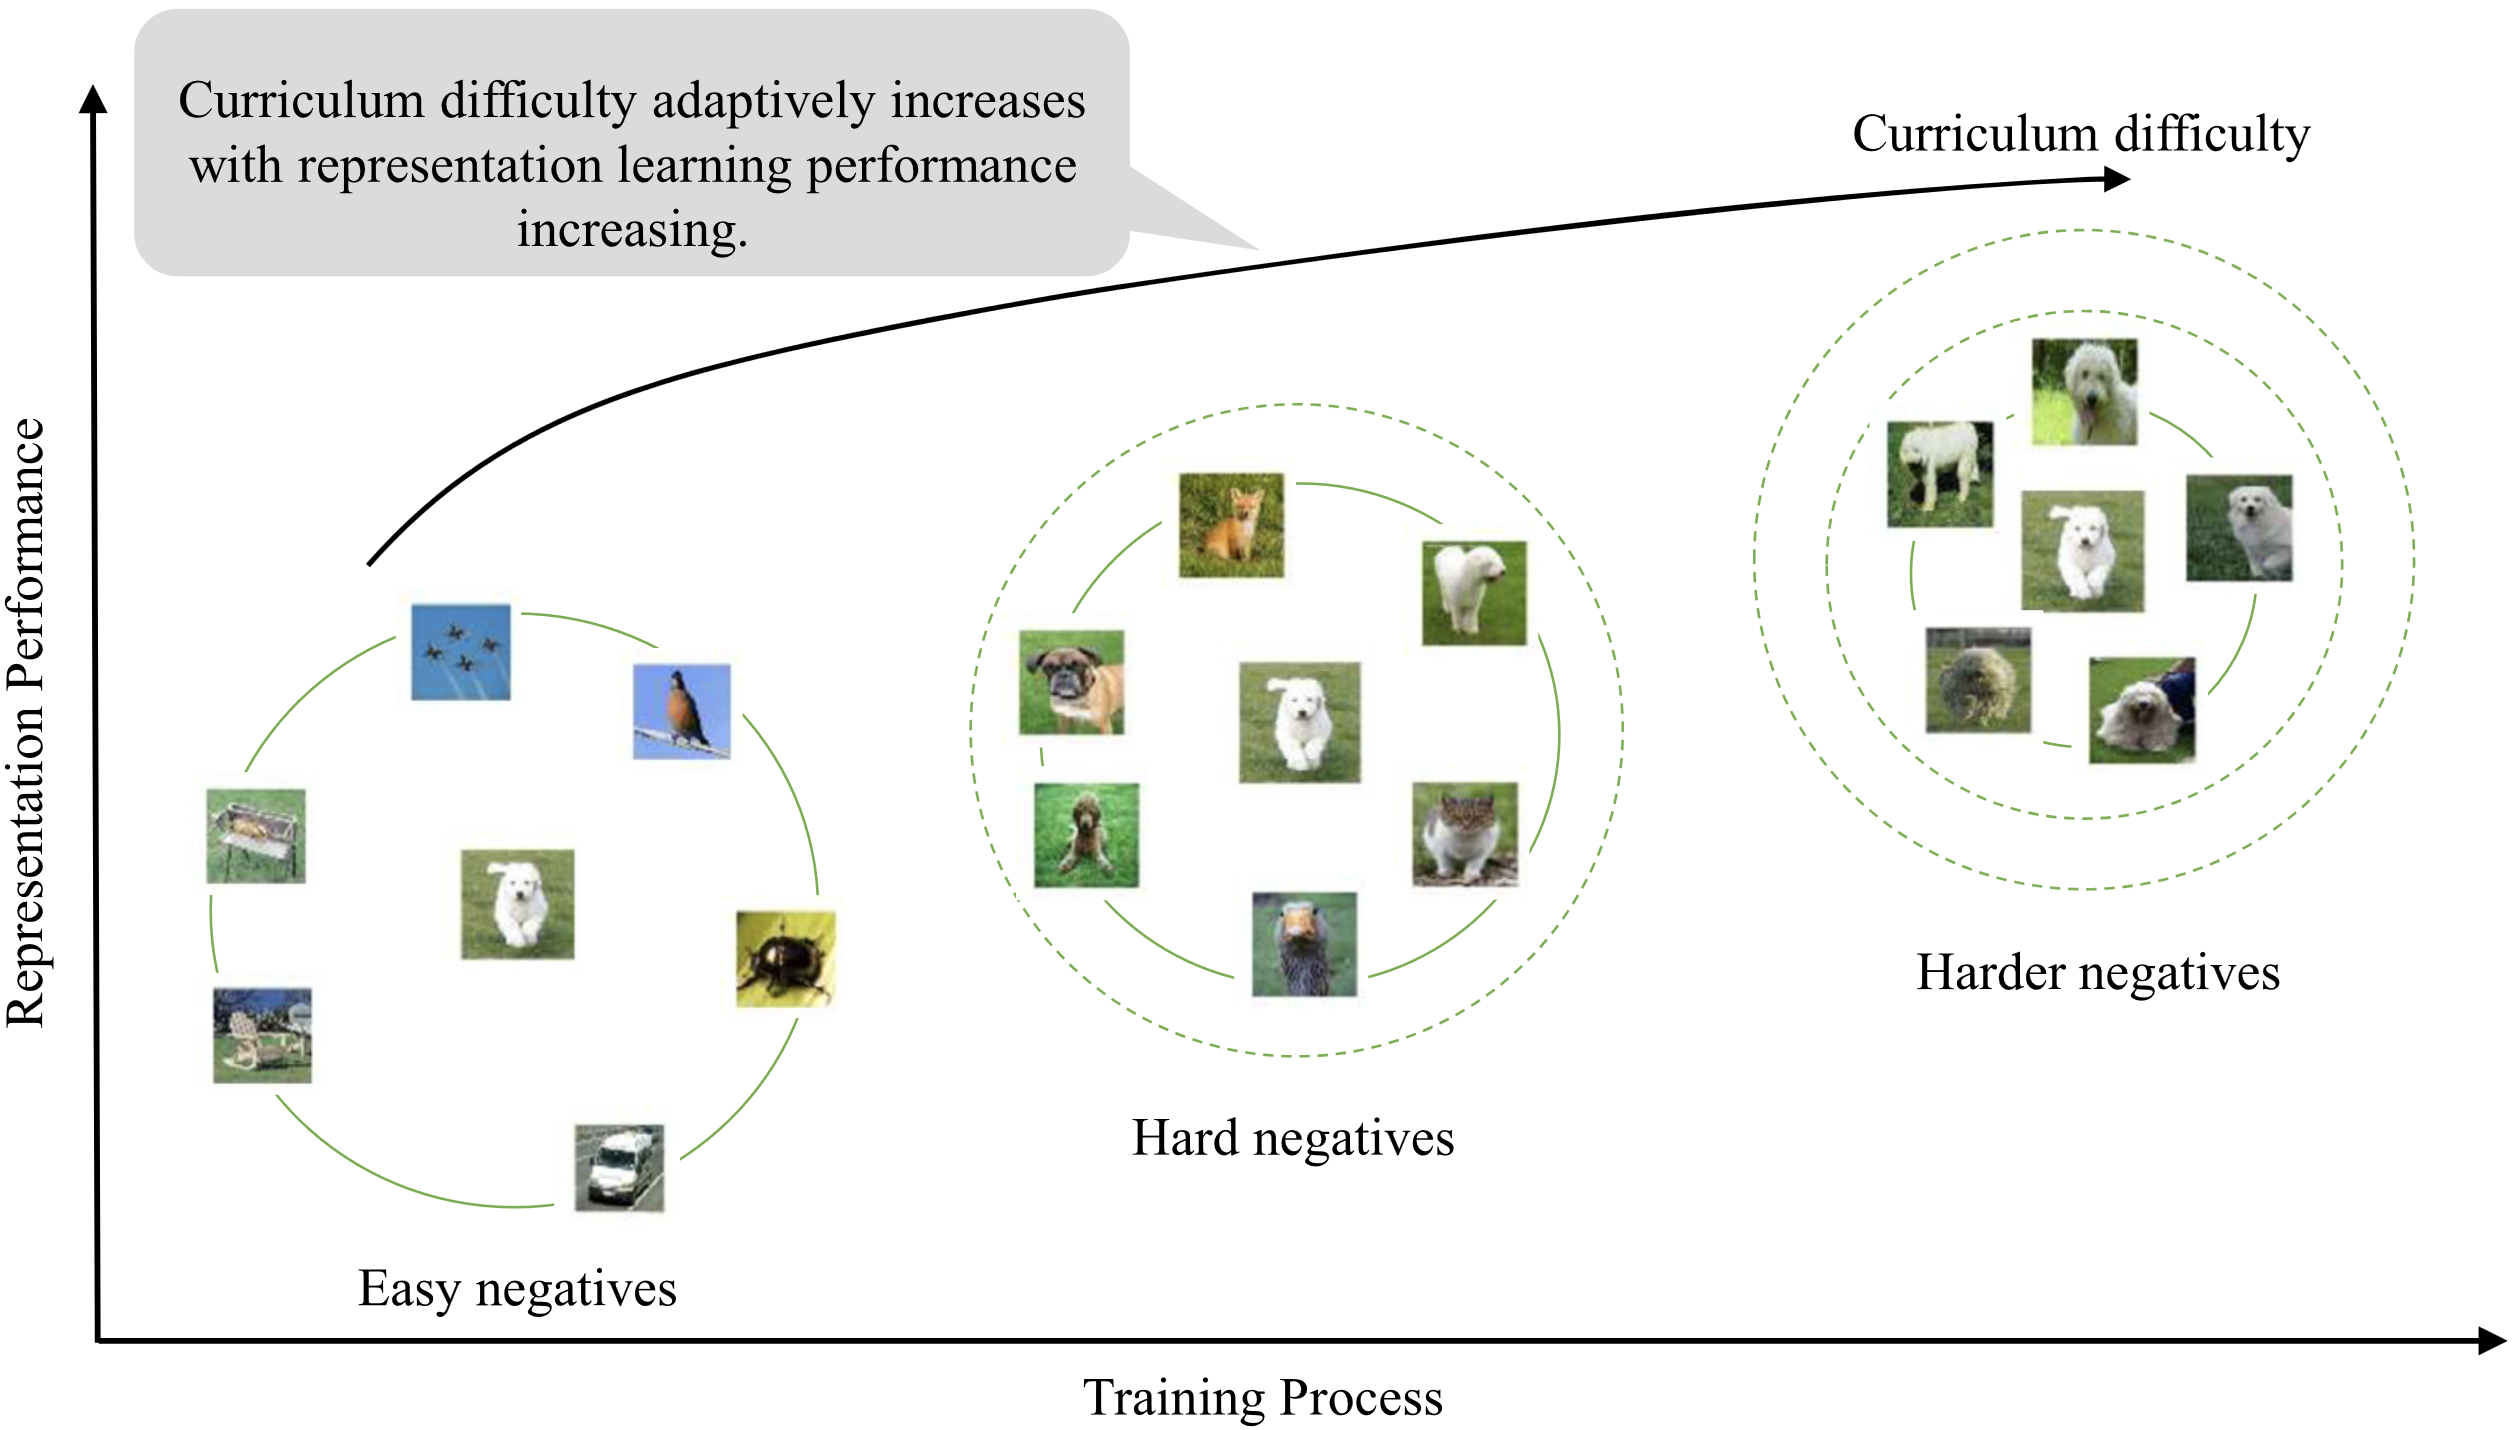
\includegraphics[width=360pt]{images/curriculum_learning_samples.png}
    \caption{Selection of negative samples for different stages of the training process 
    from \citet{curricular_weighting_2024}.
    Initially, the model is trained on easy negative samples.
    The difficulty of the negative samples is gradually increased over time.
    Solid circles represent the samples that are prioritized for training.
    }
    \label{fig:curriculum_learning_samples}
\end{figure}

This approach considers samples from the same batch that are harder to distinguish from the anchor 
than its positive sample obtained by an augmentation, hard negatives.
Firstly, the embeddings are $\mathcal{L}_2$ normalized.
Secondly, the similarity between the anchor and the other samples in the batch is calculated via the dot product.
The similarity of the positive pair is denoted as $s_{ii'}$ and the similarity of the negative pair as $s_{ij}$.
If the similarity of the negative pair is bigger than the similarity of the positive pair, 
the weight of the negative sample is multiplied by a factor $w_{ij}$ 
as illustrated in \eqref{eq:curricular_negative_weighting}.

\begin{equation}
    N(i,j,t) = \left\{\begin{array}{ll} s_{ij}, & s_{ij} \le s_{ii'} \\
        s_{ij} \cdot  w_{ij}, & s_{ij} > s_{ii'}\end{array}\right. ,\text{ where }w_{ij} = t + s_{ij}
    \label{eq:curricular_negative_weighting}
\end{equation}

$w_{ij}$ is governed by the negative pair's similarity $s_{ij}$ to emphasising hard negatives 
and the parameter $t$ which is adapted during training.
At the beginning of the training process, $t$ is set close to zero and $w_{ij} < 1$ 
to assign smaller relative weights to hard negatives.
As the training progresses, $t$ is increased to assign higher weights $w_{ij} > 1$ to hard negatives.

\begin{equation}
    r_i(j) = \frac{\left| \frac{\partial \mathcal{L}_i}{\partial s_{ij}} \right|}
    {\left| \frac{\partial \mathcal{L}_i}{\partial s_{ii'}} \right|}
    \label{eq:curricular_weighting_ratio}
\end{equation}


By calculating the ratio $r_i(j)$ of the hard negative gradient and positive gradient 
with respect to the loss for different values of $t$ by \eqref{eq:curricular_weighting_ratio}, 
the authors show that the model gradually focuses on hard negatives.
The resulting plot is depicted in \autoref{fig:gradient_ratio_hard_neg_pos}.

\begin{figure}[h] % h = here, t = top, b = bottom, p = page of floats
    \centering
    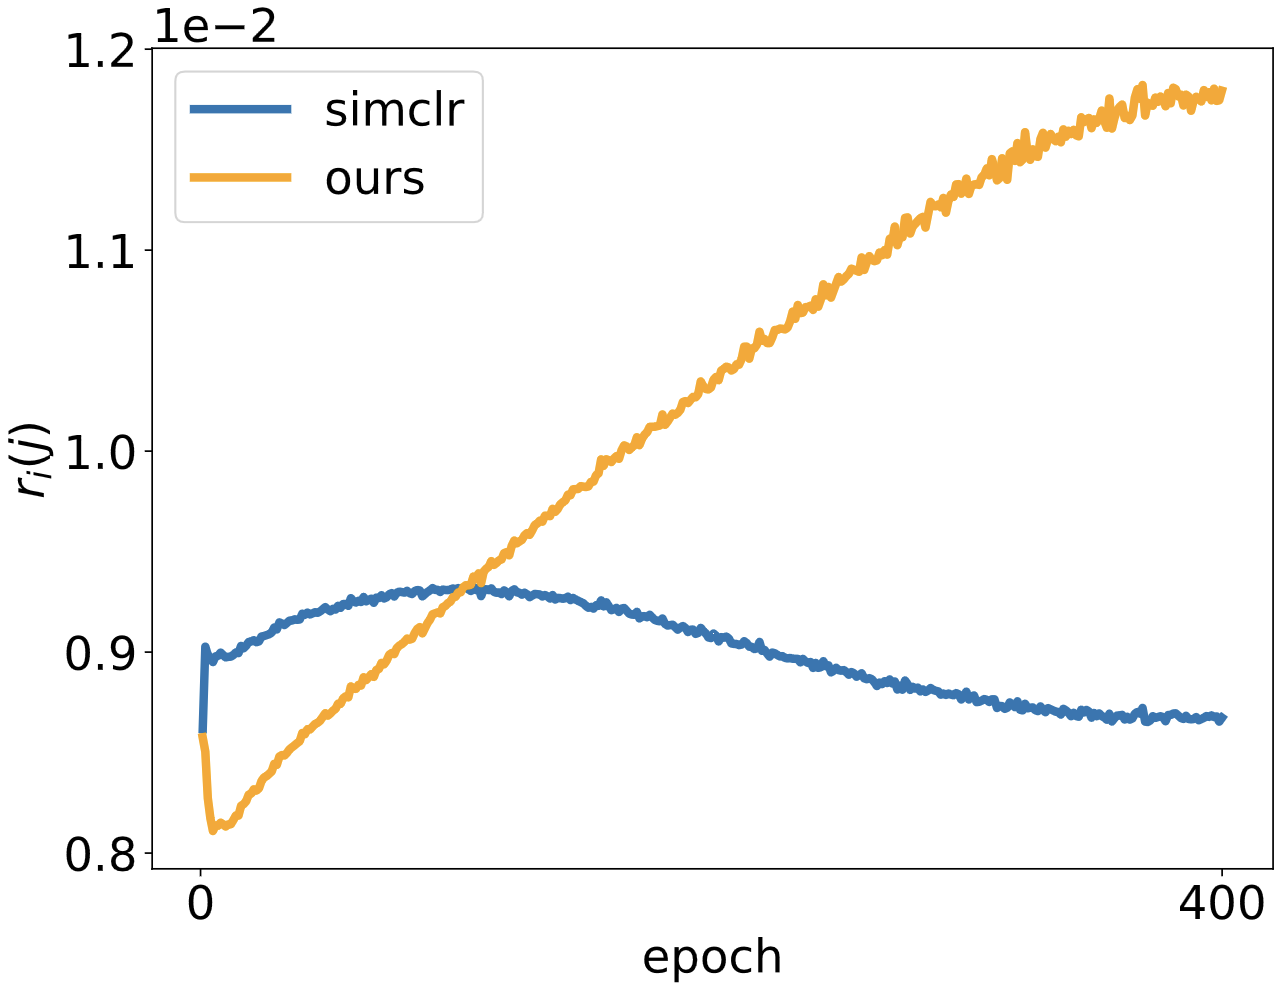
\includegraphics[width=120pt]{images/ratio_hard_neg_pos_gradients.png}
    \caption{Dispay of the gradient ratio of hard negative and positive samples (orange) throughout training 
    from \citet{curricular_weighting_2024}.
    As the training progresses, the model focuses more on hard negative samples, i.e. the ratio increases.
    }
    \label{fig:gradient_ratio_hard_neg_pos}
\end{figure}

The parameter $t$ is updated according to \eqref{eq:curricular_weighting_t_update}, where $m$ is a momentum encoder.
Intuitively, $t$ is a moving average of the average similarity of the positive pairs 
which is implicitly aligned with the model's performance. 
Since this average similarity is expected to increase over time, so will $t$ \citet{curricular_weighting_2024}.

\begin{equation}
    t^{(k)} = m \cdot t^{(k-1)} + (1-m) \cdot \frac{1}{N}\sum_{i=1}^{N}s^{k}_{ii'} 
    \label{eq:curricular_weighting_t_update}
\end{equation}

\citeauthor{curricular_weighting_2024} stress that in order to avoid losing the semantic structure of the embedding space 
due to highly weighted \acp{fn}, weights $w_{ij} > 1$ are $\mathcal{L}_2$ regularized.
They compare the model's accuracy with and without the proposed regularization approach on both the CIFAR-10 and the STL-10 datasets 
to support the usage of regularization.

% ablation study
Moreover, the authors conduct an ablation study to investigate the impact of the proposed weighting scheme 
by comparing it to fixed small and high $t$ values, as well as fixed transitions of $t$ values during training accuracy to cosine functions.
The proposed adaptive weighting scheme outperforms the fixed weighting schemes.


% ---- end section ---- 
\section{Critic}\label{sec:critic}

Even though the presented sampling techniques are very promising, after gathering and evaluating the information, 
some critical points arise which will be discussed in the following.

% positive augmentations
Many scientists have led their paper with the statement that the generation of positive samples has already been subject to many studies.
However, the majority of the papers subject to this work used random transformations to generate positive samples \citet{robinson_contrastive_2021,adversarial_2020,swav_2020}.
While the effort invested in initially identifying effective augmentation strategies for positive samples is evident, 
the consideration given to positive sample generation in these papers appears relatively superficial.

% explainable sample generation
From an explainability perspective, 
using cluster-based sample generation techniques appears to be a more promising approach 
than simply stating that a randomly selected augmentation from a set of transformations was applied, 
without providing further motivation or detail.

% manifold mining
\citet{mining_manifolds_2018}'s manifold mining approach, on the other hand, poses an interesting and more graspable approach to sample generation. 
However, according to the paper, the manifold is calculated only once at the beginning of the training process.
This is possible either due to the assumption that the manifold does not change during the training process or 
due to computational costs.
Since the manifold is calculated based on the Euclidean nearest neighbour graph which is dependent on the embedding, 
the manifold structure could change during the training process of the embedding function.
Therefore, recalculation of the manifold could be of interest.

% clustering-based approaches
Some clustering-based approaches such as \ac{pcl} \citet{PCL_2021} seem to need $M$ clusterings per iteration 
which seems computationally expensive. 
However, since a batch of samples changes the embedding, recalculation of the clusters is necessary.
Nevertheless, the computational costs of this approach should be considered when evaluating \ac{pcl}'s overall usability.

% cosine similarity
Even though most papers use the dot product to calculate the similarity between samples, 
\citet{mining_potential_2024} and \ac{la} \citet{local_aggr_2019} use cosine similarity 
without providing further justification. % do authors say why they use it? LA: No, Potential: No
The cosine similarity is a measure of the angle between two vectors and does not consider the magnitude.
Therefore, the use of cosine similarity to measure the similarity between samples appears questionable.


% high dimensional spaces
The curse of dimensionality states that in high-dimensional spaces, distances become meaningless.
Consequently, cluster-based approaches in high-dimensional spaces might not be as effective as in lower-dimensional spaces.
Since dimensionality reduction always leads to information loss, one has to consider this drawback when using clustering-based approaches 
such as \ac{drc} \citet{DRC_2020}, \ac{swav} \citet{swav_2020}, \ac{pcl} \citet{PCL_2021}, 
\ac{la} \citet{local_aggr_2019} or mining manifolds \citet{mining_manifolds_2018}.
To avoid information loss, i.e. working on the original high-dimensional data, 
the usage of approaches such as \ac{mochi} \citet{mochi_2020} seem beneficial.

% DRC & L_{ap}
The clustering-based approach \ac{drc} \citet{DRC_2020} was briefly discussed in \autoref{subsec:SampleViaClustering}.
\ac{drc} aims to address the issue of existing methods enforcing the representations of samples 
and their augmentations to be assigned to the same cluster regardless of their \ac{af}.
Hence, they consider both the \ac{af} and the \ac{ap} during clustering.
Since the \ac{ap} is calculated via the softmax function of the \ac{af}, 
it is debatable whether the usage of \ac{ap} in the loss is necessary.

\section{Own ideas}\label{sec:own_ideas}
\newcommand{\fisher}{Fisher's linear discriminant}

% clustering algos
The majority of clustering-based techniques use algorithms such as $k$-means to generate clusters.
$k$-means' implicit assumptions include that clusters are spherical, isotropic and have roughly the same numbers of samples. % = fester Radius
To loosen these assumptions, other clustering algorithms could be used.
For instance, \ac{dbscan} could be a promising alternative depending on the underlying data.
According to \citet{local_aggr_2019}, \ac{dbscan} scales well to large datasets.
Moreover, it is not necessary to specify the number of clusters $k$ beforehand and 
it is able to detect clusters of arbitrary shapes.
However, \citeauthor{local_aggr_2019} claim that \ac{dbscan} performs poorly on 
high-dimensional data or highly variable density functions.

A combination of different clustering algorithms for methods such as 
\ac{la} \citep{local_aggr_2019} or \ac{pcl} \citep{PCL_2021} could be beneficial.
Since \ac{la} employs $m$ different $k_m$ values for $k$-means, 
creating hierarchical clusters of varying granularity, 
where larger $k_m$ values produce more (granular) clusters, 
the diversity of clusters could be further enhanced by incorporating alternative clustering algorithms. 
This would introduce a broader range of cluster shapes and structures.

% AE instead of CNN
% CNNs and Autoencoders are not mutaly exclusive: CNN = architecture, VAE = Framework, can be implemented using CNNs
% Since most techniques discussed in this work have image input data \acp{cnn} seem to be a natural choice for generating embeddings.
% However, using \acp{ae} to generate embeddings could be a promising alternative.
% Since \acp{ae} are trained using the reconstruction error of the input and output, no additional data is necessary.
% This idea is purely speculative and has not been tested yet.

% shortest path in graph
If the data is clustered as displayed in \autoref{fig:graph_svm}a,
the sample pairs within a cluster that have the longest shortest path could be considered as hard positive samples.
Conversely, sample pairs in different clusters with the shortest path could be considered as hard negative samples.

\begin{figure}[!htb]%
    \centering
    \subfloat[\centering Longest shortest path pairs within a cluster are considered hard positive pairs (green) 
    while shortest path pairs of different clusters are considered hard negative (red).]
    {{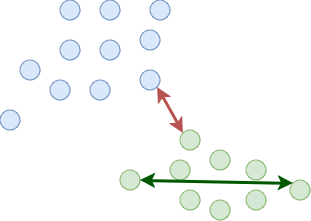
\includegraphics[width=5cm]{images/Cluster_samples.drawio.png} }}%
    \qquad
    \subfloat[\centering Visualization of the \acs{svm} approach. 
    \acsp{sv} are displayed as bold points.
    Red arrows denote (hard) negative pairs while green arrows denote (hard) positive pairs.]
    {{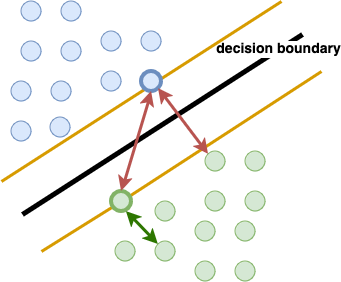
\includegraphics[width=5cm]{images/SVM_samples.png} }}%
    \caption{Samples are displayed as points and their colour denotes their cluster membership.}%
    \label{fig:graph_svm}%
\end{figure}

% SNA measures
Even if the input data is not initially a graph, one could transform it into a graph via, for instance, 
the Euclidean nearest neighbour graph discussed in \autoref{subsec:mining_manifolds}.
In computer science, \ac{sna} is a well-known field.
\ac{sna} scientists have developed many measures to analyze graphs.
Therefore, another idea is to use the concept of cliques.
A clique is a subset of vertices of an undirected graph such that every two distinct vertices in the clique are adjacent.
Vertices in a clique are easy positives and reachable vertices outside the clique are hard positives.
This idea would consider the clique vertices to be interchangeable.

% SVM: SV as negative samples
Another idea is to use \acfp{svm} to generate (hard) samples as visualized in \autoref{fig:graph_svm}b.
Initially, the data is split into two classes. 
Since true class labels are not available in \ac{cl}, clustering results are used as a proxy.
Then, a \ac{svm} is trained on the data.
After training, the decision boundary is determined such that 
the margin between the clusters is maximal.
The samples that are closest to the decision boundary are considered as \acfp{sv}.
Each pair of \acp{sv} from different sides of the decision boundary is considered a hard negative pair.
Similarly, distant samples from the decision boundary and their \acp{sv} are considered (hard) positive pairs.
% Since \ac{svm} is a binary classifier, $k>2$ clusters have to be handled via
% multiple one-vs-the-rest or one-vs-one approaches.

\begin{figure}[!htb]%
    \centering
    \subfloat[\centering Visualization of the \fisher{} approach.
    To facilitate visualization, the projection of the samples is only implied by dotted lines 
    but not displayed explicitly.
    Overlapping projected samples (bold circles) of different clusters are considered hard negative pairs.]
    {{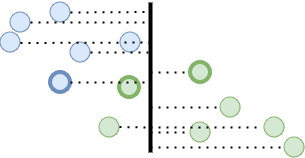
\includegraphics[width=6cm]{images/Fishers_linear_discriminat_samples.drawio.png} }}%
    \qquad
    \subfloat[\centering Display of the \ac{pca} idea.
    The first two \ac{pca} axes of each cluster are displayed as lines.
    Green arrows denote positive pairs while red arrows denote negative pairs.]
    {{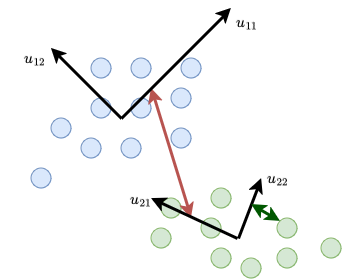
\includegraphics[width=4cm]{images/PCA_samples.png} }}%
    \caption{Samples are displayed as points and their colour denotes their cluster membership.}%
    \label{fig:fisher_pca}%
\end{figure}

% Fisher's linear discriminant: overlapping samples
It may be possible to use \fisher{} to generate hard negative samples.
\fisher{} is a linear projection that maximizes the distance between the means of the classes.
Again, two classes are determined via clustering.
As visualized in \autoref{fig:fisher_pca}a, the projected samples of different classes that 
are closest to each other are considered negative samples.

% different PCA axes as negative samples
Since \ac{pca} is a linear transformation, that maximizes the variance of projected data, 
it is the best linear dimension reduction technique in terms of minimization of information loss.
Again, multiple classes are determined via clustering.
The first $n$ \ac{pca} axes are determined for each cluster.
% axes points as samples
Since these axes explain the most variance, equidistant samples lying on these axes could be used as generated samples.
Projected samples and their corresponding generated axis samples are treated as positive samples, 
while projected samples and axes samples from other clusters are considered negative samples.
This idea is visualized in \autoref{fig:fisher_pca}b.
% cosine similarity
An alternative approach could be to use cosine similarity between vectors spanning \ac{pca} axes of different clusters 
rather than the dot product of two samples belonging to different clusters, 
because the magnitude of the axes is not of interest but only their direction.

% curriculum learning: different sample generation techniques
Moreover, the concept of curricular weighting proposed in \autoref{subsec:curricular_weighting} could be extended.
The notion of hard negative samples being samples in the batch that are more similar to the anchor than positive samples 
proposed in \citet{curricular_weighting_2024} is only one version to generate hard negative samples.
Using other sample generation techniques discussed in this work in combination with 
the idea of gradually increasing the level of hardness during training could be beneficial.

% drawbacks of ideas: initial clustering
The main drawback of the ideas presented in this section is the initial clustering.
If this clustering produces poor results, i.e. the cluster's samples have different inherent labels, 
all proposed ideas will produce \acp{fn} and thus, the training process will be negatively affected.

% drawbacks of ideas: k>2 clusters
Another issue is working on $k>2$ clusters when using either the \ac{svm} or the \fisher{} approach.
Both techniques are originally designed for binary classification problems.
In order to extend the ideas to multi-class problems, one-vs-one or one-vs-all approaches have to be used. 
These extensions are prone to ambiguities during inference and 
come with additional computational effort.

% end
The exploration of various \ac{cl} techniques has demonstrated their effectiveness in \ac{ssl}, 
particularly in producing high-performing models trained on unlabelled data. 
Despite the promising results, challenges remain, such as optimizing the selection of negative and positive samples 
and improving computational efficiency.

\section*{Usage of generative AI and AI-assisted technologies}
\label{sec:usage_AI}
% Use of Language Assistance Tools

I hereby declare that I used ChatGPT and Grammarly for rewording and spelling correction purposes. 
These tools assisted me in enhancing the clarity and accuracy of the text.

\section*{Declaration of originality}
\label{sec:dec_originality}

I declare that this paper is entirely my
original work unless otherwise indicated and properly cited. 
This declaration encompasses all aspects of
the paper, including but not limited to text, figures, tables, data, and any accompanying materials.
\newline

\noindent \underline{ \hspace{6cm}} 
\\ Kassel, \today \hspace{1cm}


% ---- Bibliography ----
\bibliographystyle{unsrtnat}
\bibliography{references}

% ---- Acronyms ----
\newpage
\section*{General acronyms}
\begin{acronym}

    \acro{nn}[NN]{Neural Network}
    \acro{cl}[CL]{Contrastive Learning}
    \acro{gcl}[GCL]{Graph Contrastive Learning}
    \acro{pu}[PU]{Positive-Unlabeled}
    \acro{fn}[FN]{False Negative}
    %\acro{fp}[FP]{False Positive}
    \acro{tn}[TN]{True Negative}
    \acro{ssl}[SSL]{Self-Supervised Learning}
    %\acro{fgsm}[FGSM]{Fast Gradient Sign Method}
    \acro{af}[AF]{Assignment Feature}
    \acro{ap}[AP]{Assignment Probability}
    \acro{cnn}[CNN]{Convolutional Neural Network}
    %\acro{moco}[MoCo]{Momentum Contrast}
    \acro{em}[EM]{Expectation-Maximization}
    %\acro{pic}[PIC]{Parametric Instance Classification}
    \acro{bmm}[BMM]{beta mixture model}

\end{acronym}

\section*{\ac{cl} approach-specific acronyms}
\begin{acronym}

    %\acro{clae}[CLAE]{Contrastive Learning with Adversarial Examples}
    \acro{drc}[DRC]{Deep Robust Clustering}
    \acro{la}[LA]{Local Aggregation}
    \acro{mochi}[MoCHi]{Mixing of Contrastive Hard negatIves}
    \acro{pcl}[PCL]{Prototypical Contrastive Learning}
    \acro{swav}[SwAV]{Swapping Assignments between multiple Views of the same image}
    %\acro{grape}[GRAPE]{Graph contrastive learning via subspace preserving}
    % \acro{psm}[PSM]{Potential Sample Mining}
    % \acro{ppsm}[PPSM]{Potential Positive Sample Mining}
    % \acro{pnsm}[PNSM]{Potential Negative Sample Mining}
    \acro{aas}[AAS]{Authority-Ascent Shift}

\end{acronym}

\end{document}
